\documentclass{article}
\usepackage{amsmath,amssymb,amstext,amsfonts}
\usepackage{color}
\usepackage{url}
\usepackage{algorithmic,algorithm}	
\usepackage{listings} 
	% Python style for highlighting
	\newcommand\pythonstyle{\lstset{
	language=Python,
	basicstyle=\ttm,
	otherkeywords={self},             % Add keywords here
	keywordstyle=\ttb\color{deepblue},
	emph={MyClass,__init__},          % Custom highlighting
	emphstyle=\ttb\color{deepred},    % Custom highlighting style
	stringstyle=\color{deepgreen},
	frame=tb,                         % Any extra options here
	showstringspaces=false            % 
	}}
	% Python environment  % use \begin{python} \end{python}
	\lstnewenvironment{python}[1][]
	{
	\pythonstyle
	\lstset{#1}
	}
	{}
	% Python for external files
	\newcommand\pythonexternal[2][]{{
	\pythonstyle
	\lstinputlisting[#1]{#2}}}
	% Python for inline
	\newcommand\pythoninline[1]{{\pythonstyle\lstinline!#1!}}

\usepackage[pdftex]{graphicx}
  \graphicspath{{figures/}}
  \DeclareGraphicsExtensions{.pdf,.jpg,.jpeg,.png}
  
%\usepackage{pdfpages} % to include pdf documents
  
\usepackage[english]{babel}
\usepackage{amsthm}
\newtheorem{theorem}{Theorem}[section]
\newtheorem{lemma}[theorem]{Lemma}
\newtheorem{example}[theorem]{Example}
\newtheorem{definition}[theorem]{Definition}
\newtheorem{corollary}[theorem]{Corollary}
  

\newcommand{\norm}[1]{\left\|{#1}\right\|}
\newcommand{\abs}[1]{\left|{#1}\right|}
%\newcommand{\defeq}{\stackrel{\triangle}{=}}
\newcommand{\defeq}{\circeq}
\newcommand{\fov}[1]{\text{\em fov}\left(#1\right)}
\newcommand{\fovinv}[1]{\text{\em fov}^{-1}\left(#1\right)}
\newcommand{\odd}[1]{\text{\em odds}\left(#1\right)}
\renewcommand{\vec}[1]{\text{\em vec}\left(#1\right)}
\newcommand{\bbf}{\mathbf{b}}
\newcommand{\cbf}{\mathbf{c}}
\newcommand{\pbf}{\mathbf{p}}
\newcommand{\sbf}{\mathbf{s}}
\newcommand{\ubf}{\mathbf{u}}
\newcommand{\xbf}{\mathbf{x}}
\newcommand{\onebf}{\mathbf{1}}
\newcommand{\Cbf}{\mathbf{C}}
\newcommand{\Ibf}{\mathbf{I}}
\newcommand{\Pbf}{\mathbf{P}}
\newcommand{\phibf}{\boldsymbol{\phi}}
\newcommand{\mubf}{\boldsymbol{\mu}}
\newcommand{\xibf}{\boldsymbol{\xi}}
\newcommand{\sigmabf}{\boldsymbol{\sigma}}
\newcommand{\Pibf}{\boldsymbol{\Pi}}
\newcommand{\Sigmabf}{\boldsymbol{\Sigma}}

\newcommand{\TODO}[1]{{\color{red}#1}}
\newcommand{\rwbcomment}[1]{{\color{blue}RWB: #1}}


\title{\LARGE \bf
B-Splines for Robotic Applications
}
\date{Updated: \today}

\author{Randal~W.~Beard \\ Brigham Young University}

\begin{document}

\maketitle

\begin{abstract}
These notes provide an overview of B-splines and their applications to robotics.  In particular, we have in mind applications to path planning for aerial vehicles, model predictive control, and fixed-lag state estimation.  
\end{abstract}

%---------------------------------------------------------------
\section{Motivation}

The objective of these notes is to explore spline methods for robotic applications. In general, the position of a robot in Euclidian space can be described by a time parametrized trajectory $\mathbf{p}(t)\in\mathbb{R}^3$, $t\in[a,b]$.  The time parametrized trajectory can be parameterized using a weighted sum of basis function as
\[
\mathbf{p}(t) = \sum_{m=0}^{N} \cbf_m \phi_m(t),
\]
where $\cbf_m\in\mathbb{R}^n$, and $\phi_m(t)$ are a set of basis functions.  For example, the basis functions could be the set of polynomial power function $\phi_m(t) = t^m/m!$, or the set of sinusoidal function $\phi_m(t) = \sin(\frac{2\pi m}{N}t)$.  The disadvantage of both the polynomial power functions and sinusoidal functions is that the basis functions are defined for all $t\in[a,b]$ and so each control points $\mathbf{c}_m$ influences the entire trajectory.  Another disadvantage is that a large number of basis functions may be required to represent complicated trajectories.  

In these notes, we will use B-spline basis functions which have a number of very nice properties that we will explore.  In particular, a {\em B-spline} trajectory has the following form
\[
\mathbf{p}(t) = \sum_{m=0}^{N} \cbf_m b_m^k(t;\mathbf{t}),
\]
where $\cbf_m\in\mathbb{R}^n$ are the control points,  $\mathbf{t}=(\tau_0, \tau_1, \tau_2, \dots, \tau_T)$ are called the knot points where $i<j \implies \tau_i\leq \tau_j$, and $b_m^k(t;\mathbf{t})$ are the B-spline basis functions of order $k$. The spline trajectories will be defined for $t$ in the span of the knot points, i.e., $t\in[\tau_0, \tau_T]$.  

Section~\ref{sec:b-spline-basis-functions} defines the B-spline basis function $b_m^k(t; \mathbf{t})$ and describes some of their properties that will be useful for path planning and for estimation.
Section~...
% overview of other sections

%---------------------------------------------------------------
\section{B-Spline Basis Functions}
\label{sec:b-spline-basis-functions}

The B-spline basis function are defined by the recursive formula:
\begin{align}
b_m^0(t; \mathbf{t}) &= \begin{cases} 1 & \text{~if~} \tau_m \leq t \leq \tau_{m+1} \\ 
 									 0 & \text{~otherwise} 
 					   \end{cases} 
	\label{eq:spline_basis_definition_0}\\	
b_m^k(t; \mathbf{t}) &= \frac{t-\tau_m}{\tau_{m+k}-
\tau_m} b_m^{k-1}(t; \mathbf{t}) + \frac{\tau_{m+k+1}-t}{\tau_{m+k+1}-\tau_{m+1}} b_{m+1}^{k-1}(t; \mathbf{t}),
	\label{eq:spline_basis_definition_k}
\end{align}
where by convention, a divide by zero in Equation~\eqref{eq:spline_basis_definition_k} is interpreted to mean that the associated term is zero.

%+++++++++++++++++++++++++++++++
\subsection{Zeroth order basis}

For example, if the knot vector is given by
\[
\mathbf{t} = [\tau_0, \tau_1, \tau_2] \defeq [0, 1, 2],
\]
then there are two basis function of order $k=0$ given by
\begin{align*}
b_0^0(t; \mathbf{t}) &= \begin{cases} 1 & \text{~if~} \tau_0 \leq t \leq \tau_1 \\ 
 									 0 & \text{~otherwise} 
 			\end{cases}
\\ 
b_1^0(t; \mathbf{t}) &= \begin{cases} 1 & \text{~if~} \tau_1 \leq t \leq \tau_2 \\ 
 									 0 & \text{~otherwise}
 			\end{cases}
\end{align*}
where $b_0^0(t)$ and $b_1^0(t)$ are shown in Figure~\ref{fig:spline_basis_0}.
\begin{figure}[hbt]
  \centering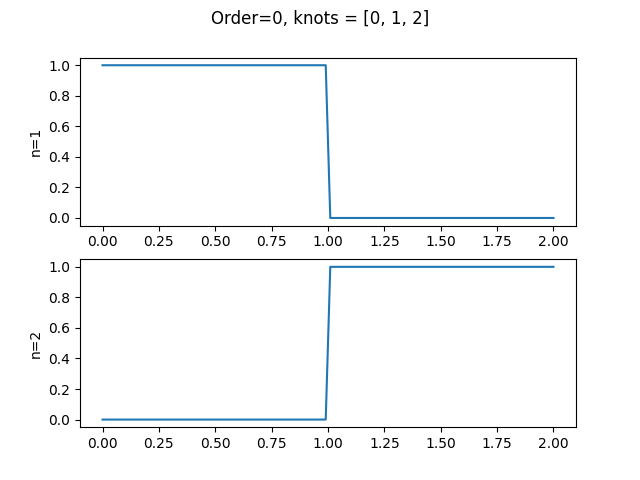
\includegraphics[width=0.5\textwidth]{./figures/spline_basis_0}
  \caption{Zeroth order spline basis}
  \label{fig:spline_basis_0}  
\end{figure}
Note that $b_1^0(t; \mathbf{t}) = b_0^0(t-1; \mathbf{t})$, or in other words, all zeroth order basis functions are shifted versions of the central zeroth order basis function $b_0^0(t; \mathbf{t})$.  Additional zeroth order basis function can be defined by expanding the knot vector to $\mathbf{t}=[0, \dots, M]$, where $b_m^0(t; \mathbf{t})= b_0^0(t-m; \mathbf{t})$ for $m\leq M$.

\clearpage


%+++++++++++++++++++++++++++++++
\subsection{First order basis}

If the knot vector is given by
\[
\mathbf{t} = [\tau_0, \tau_1, \tau_2, \tau_3, \tau_4] \defeq [0, 0, 1, 2, 2],
\]
then there are $2k+1=3$ unique basis function of order $k=1$ given by
\begin{align*}
b_0^1(t; \mathbf{t}) &= \frac{t-\tau_0}{\tau_1-\tau_0} b_0^0(t;\mathbf{t}) + \frac{\tau_2-t}{\tau_2-\tau_1}b_1^0(t; \mathbf{t}) 
	= \begin{cases} 0   & \text{~if~} t_0=0 \leq t \leq t_1=0 \\
				    1-t & \text{~if~} t_1=0 \leq t \leq t_2=1 \\ 
 	  \end{cases}
\\ 
b_1^1(t; \mathbf{t}) &= \frac{t-\tau_1}{\tau_2-\tau_1} b_1^0(t;\mathbf{t}) + \frac{\tau_3-t}{\tau_3-\tau_2}b_2^0(t; \mathbf{t})
	= \begin{cases} t & \text{~if~} t_1=0 \leq t \leq t_2=1 \\ 
 									2-t & t_2=1 \leq t \leq t_3=2 \\
 									0 & \text{~otherwise}
 					    \end{cases}
\\ 
b_2^1(t; \mathbf{t}) &= \frac{t-\tau_2}{\tau_3-\tau_2} b_2^0(t;\mathbf{t}) + \frac{\tau_4-t}{\tau_4-\tau_3}b_3^0(t; \mathbf{t})
	= \begin{cases} t-1 & \text{~if~} t_2=1 \leq t \leq t_3=2 \\ 
 					0 & \text{~if~} t_3=2 \leq t \leq t_4=2 \\
 	  \end{cases}
\end{align*}
where $b_0^1(t; \mathbf{t})$, $b_1^1(t; \mathbf{t})$, and $b_2^1(t; \mathbf{t})$ are shown on the left in Figure~\ref{fig:spline_basis_1}.
\begin{figure}[hbt]
  \centering
  	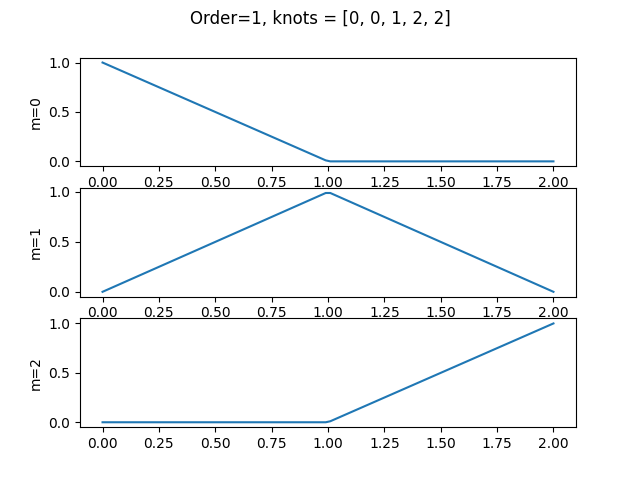
\includegraphics[width=0.45\textwidth]{./figures/spline_basis_1}
  	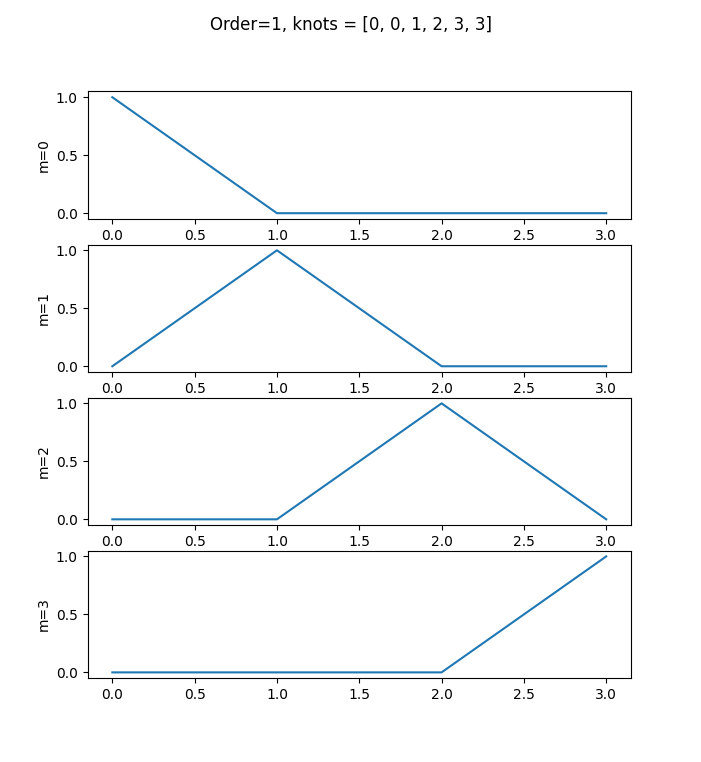
\includegraphics[width=0.45\textwidth]{./figures/spline_basis_1_extra_knot}
  \caption{First order spline basis}
  \label{fig:spline_basis_1}  
\end{figure}
If the knot vector is expanded by one time unit to
\[
\mathbf{t}' = [\tau_0, \tau_1, \tau_2, \tau_3, \tau_4, \tau_5] \defeq [0, 0, 1, 2, 3, 3],
\]
then there are still only three unique basis vectors, but 
$b_2^1(t; \mathbf{t}')$ is a shifted version $b_1^1(t; \mathbf{t})$ and $b_3^1(t; \mathbf{t}')$ is a shifted version $b_2^1(t; \mathbf{t})$, as shown on the right in Figure~\ref{fig:spline_basis_1}.

\clearpage


%+++++++++++++++++++++++++++++++
\subsection{Second order basis}

If the knot vector is given by
\[
\mathbf{t} = [\tau_0, \tau_1, \tau_2, \tau_3, \tau_4, \tau_5, \tau_6, \tau_7, \tau_8] \defeq [0, 0, 0, 1, 2, 3, 3, 3],
\]
then there are $2k+1=5$ unique basis function of order $k=2$ given by
\begin{align*}
b_0^2(t; \mathbf{t}) &= \frac{t-\tau_0}{\tau_2-\tau_0} b_0^1(t;\mathbf{t}) + \frac{\tau_3-t}{\tau_3-\tau_1}b_1^1(t; \mathbf{t}) 
	= \begin{cases} (1-t)^2   & \text{~if~} 0 \leq t \leq 1 \\
				    0 & \text{~otherwise~}  \\ 
 	  \end{cases}
\\ 
b_1^2(t; \mathbf{t}) &= \frac{t-\tau_1}{\tau_3-\tau_1} b_1^1(t;\mathbf{t}) + \frac{\tau_4-t}{\tau_4-\tau_2}b_2^1(t; \mathbf{t})
	= \begin{cases} t(2-\frac{3}{2}t) & \text{~if~} 0 \leq t \leq 1 \\ 
 									\frac{(2-t)^2}{2} & 1 \leq t \leq 2 \\
 									0 & \text{~otherwise}
 					    \end{cases}
\\ 
b_2^2(t; \mathbf{t}) &= \frac{t-\tau_2}{\tau_4-\tau_2} b_2^1(t;\mathbf{t}) + \frac{\tau_5-t}{\tau_5-\tau_3}b_3^1(t; \mathbf{t})
	= \begin{cases} \frac{t^2}{2} & \text{~if~} 0 \leq t \leq 1 \\ 
 					-\frac{3}{2}t^2 + \frac{7}{2}t - \frac{3}{2} & \text{~if~} 1 \leq t \leq 2 \\
 					\frac{(3-t)^2}{2} & \text{~if~} 2 \leq t \leq 3 \\
 					0 & \text{~otherwise}
 	  \end{cases}
\\ 
b_3^2(t; \mathbf{t}) &= \frac{t-\tau_2}{\tau_4-\tau_2} b_2^1(t;\mathbf{t}) + \frac{\tau_5-t}{\tau_5-\tau_3}b_3^1(t; \mathbf{t})
	= \begin{cases} \frac{(t-1)^2}{2} & \text{~if~} 1 \leq t \leq 2 \\ 
 					-\frac{3}{2}t^2 + \frac{15}{2}t-\frac{15}{2} & \text{~if~} 2 \leq t \leq 3 \\
 					0 & \text{~otherwise}
 	  \end{cases}
\\ 
b_4^2(t; \mathbf{t}) &= \frac{t-\tau_2}{\tau_4-\tau_2} b_2^1(t;\mathbf{t}) + \frac{\tau_5-t}{\tau_5-\tau_3}b_3^1(t; \mathbf{t})
	= \begin{cases} (t-2)^2 & \text{~if~} 2 \leq t \leq 3 \\ 
 					0 & \text{~otherwise}
 	  \end{cases}.	   	  
\end{align*}
The the unique second order basis function are shown on the left in Figure~\ref{fig:spline_basis_2}.
\begin{figure}[hbt]
  \centering
  	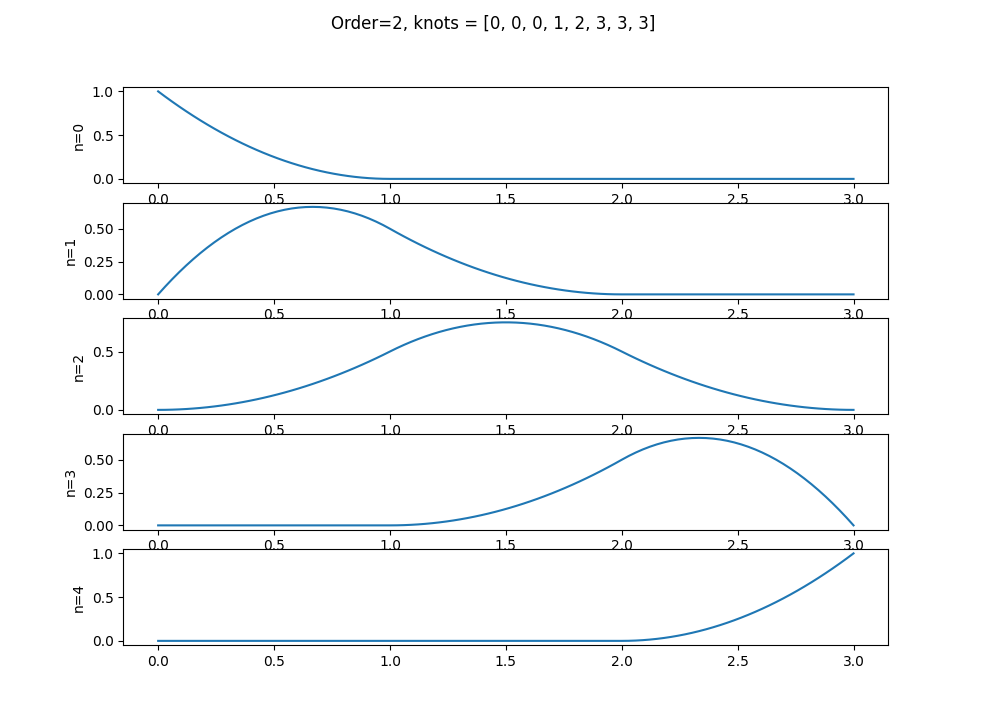
\includegraphics[width=0.45\textwidth]{./figures/spline_basis_2}
  	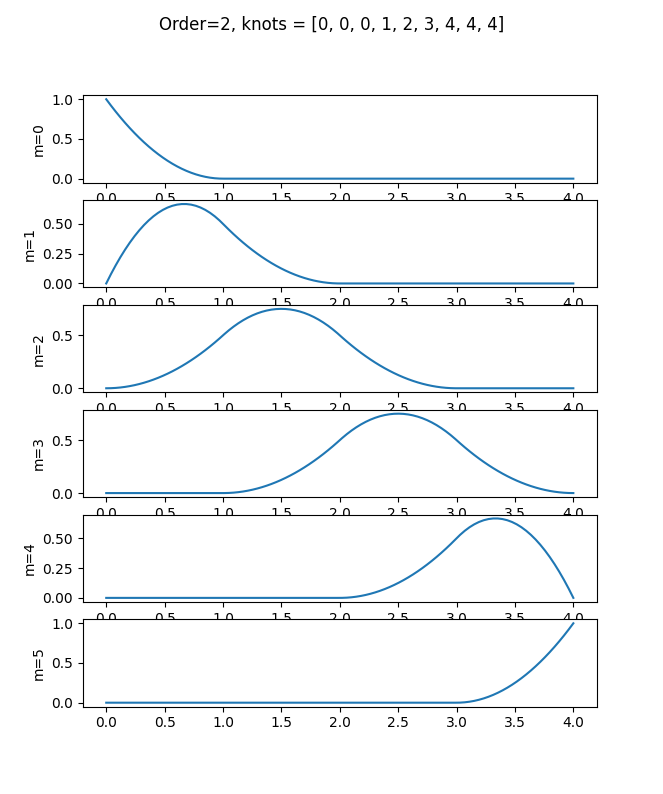
\includegraphics[width=0.45\textwidth]{./figures/spline_basis_2_extra_knot}
  \caption{Second order spline basis}
  \label{fig:spline_basis_2}  
\end{figure}
Expanding the knot vector by one time unit to 
\[
\mathbf{t}' = [\tau_0, \tau_1, \tau_2, \tau_3, \tau_4, \tau_5] \defeq [0, 0, 0, 1, 2, 3, 4, 4, 4],
\]
still results in $2k+1$ unique basis vectors, but $b_3^2(t; \mathbf{t}')$ is a right-shifted version of $b_2^2(t; \mathbf{t})$, and $b_4^2(t; \mathbf{t}')$ and $b_5^2(t; \mathbf{t})$ are a right-shifted versions of $b_3^2(t; \mathbf{t}')$ and $b_4^2(t; \mathbf{t})$, as shown on the right in Figure~\ref{fig:spline_basis_2}.

Similarly, the unique third order and eighth order basis functions are shown in Figures~\ref{fig:spline_basis_3} and~\ref{fig:spline_basis_8} respectively.

\begin{figure}[hbt]
  \centering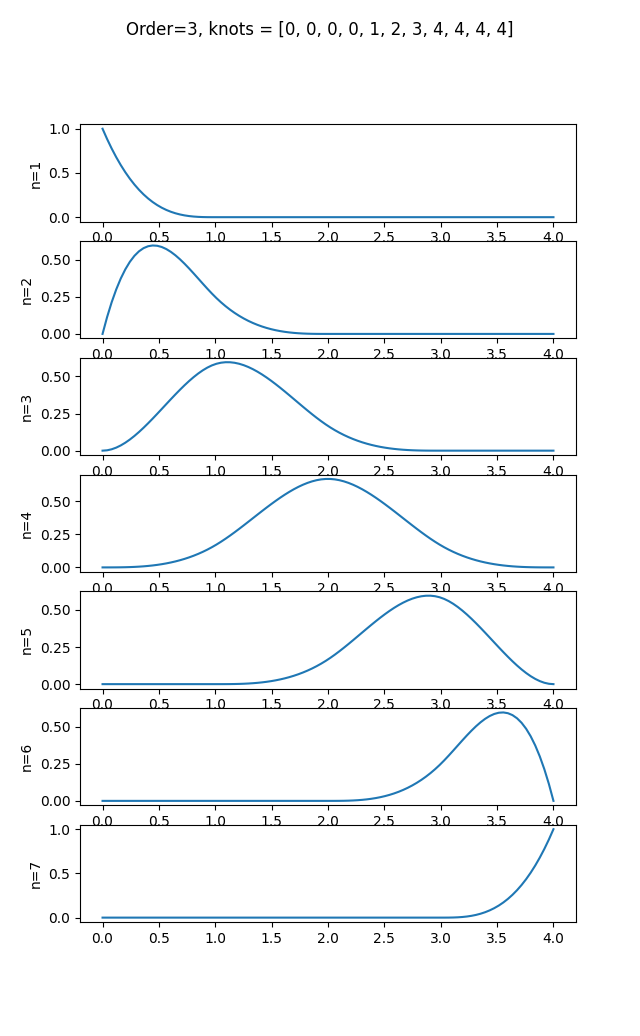
\includegraphics[width=0.99\textwidth]{./figures/spline_basis_3}
  \caption{Third order spline basis}
  \label{fig:spline_basis_3}  
\end{figure}

\begin{figure}[hbt]
  \centering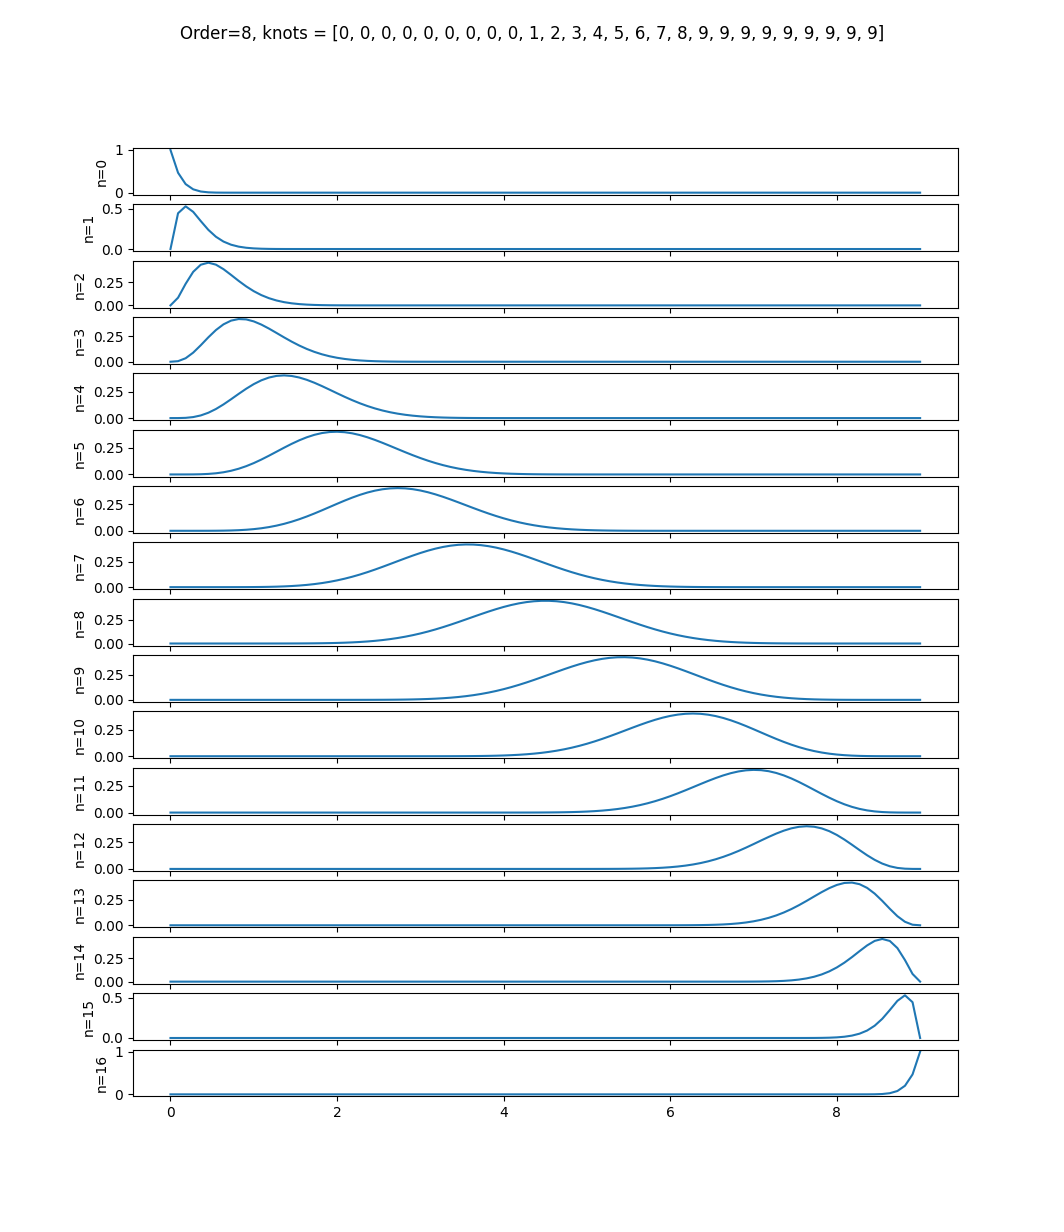
\includegraphics[width=0.99\textwidth]{./figures/spline_basis_8}
  \caption{Eighth order spline basis}
  \label{fig:spline_basis_8}  
\end{figure}

\clearpage

%---------------------------------------------------------------
\subsection{Shift and Scale Invariance of the Knot Sequence}

\begin{lemma} \label{lem:basis_are_shift_invariant}
Given an arbitrary knot sequence
\[
\mathbf{t} = [\tau_0, \tau_1, \dots \tau_T],
\]
an arbitrary time shift $\Delta$, and the one-sequenc $\mathbf{1}\defeq[1, 1, \dots, 1]$, the B-spline basis functions are shift invariant in the sense that
if 
\[
\mathbf{t} + \Delta\mathbf{1} = [\tau_0+\Delta, \tau_1+\Delta, \dots \tau_T+\Delta]
\]
then
\[
b_j^k(t; \mathbf{t}+\Delta\mathbf{1}) = b_j^k(t-\Delta; \mathbf{t}),
\]
i.e., shifting the knot sequence forward in time is identical to shifting the original B-spline forward in time.
\end{lemma}
\begin{proof}
When the order is $k=0$, then equation~\eqref{eq:spline_basis_definition_0} gives
\begin{align*}
	b_j^0(t; \mathbf{t}+\Delta\mathbf{1}) &= \begin{cases} 1 & \text{~if~} \tau_j+\Delta \leq t \leq \tau_{j+1}+\Delta \\ 
 									 				   0 & \text{~otherwise} 
 					   					 \end{cases} \\
 					   				   &= \begin{cases} 1 & \text{~if~} \tau_j \leq t-\Delta \leq \tau_{j+1} \\ 
 									 				   0 & \text{~otherwise} 
 					   					 \end{cases} \\ 	
 					   				   &= b_j^0(t-\Delta; \mathbf{t}).
\end{align*}
Assuming that the statement holds when the order is $k-1\geq 0$, we get from 
Equation~\eqref{eq:spline_basis_definition_k} that
\begin{align*}
b_j^k(t; \mathbf{t}+\Delta\mathbf{1}) &= \frac{t-\tau_j-\Delta}{\tau_{j+k}+\Delta-
\tau_j-\Delta} b_j^{k-1}(t; \mathbf{t}+\Delta\mathbf{1}) + \frac{\tau_{j+k+1}+\Delta-t}{\tau_{j+k+1}+\Delta-\tau_{j+1}-\Delta} b_{j+1}^{k-1}(t; \mathbf{t}+\Delta\mathbf{1}) \\
&= \frac{(t-\Delta)-\tau_j}{\tau_{j+k}-
\tau_j} b_j^{k-1}(t-\Delta; \mathbf{t}) + \frac{\tau_{j+k+1}-(t-\Delta)}{\tau_{j+k+1}-\tau_{j+1}} b_{j+1}^{k-1}(t-\Delta; \mathbf{t}) \\
&= b_j^k(t-\Delta; \mathbf{t}).
\end{align*}
The proof therefore follows by induction.
\end{proof}


\begin{lemma}\label{lem:bases_are_scale_invariant}
Given an arbitrary knot sequence
\[
\mathbf{t} = [\tau_0, \tau_1, \dots \tau_T]
\]
and an arbitrary scaling constant $\alpha\in\mathbb{R}$, the B-spline basis functions are scale invariant in the sense that
if 
\[
\alpha\mathbf{t} = [\alpha\tau_0, \alpha\tau_1, \dots \alpha\tau_T]
\]
then
\[
b_j^k(t; \alpha\mathbf{t}) = b_j^k(t/\alpha; \mathbf{t}),
\]
i.e., scaling the knot sequence by $\alpha$ is identical to time scaling the original B-spline by $\frac{1}{\alpha}$.
\end{lemma}
\begin{proof}
When the order is $k=0$, then equation~\eqref{eq:spline_basis_definition_0} gives
\begin{align*}
	b_j^0(t; \alpha\mathbf{t}) &= \begin{cases} 1 & \text{~if~} \alpha\tau_j \leq t \leq \alpha\tau_{j+1} \\ 
 									 				   0 & \text{~otherwise} 
 					   					 \end{cases} \\
 					   				   &= \begin{cases} 1 & \text{~if~} \tau_j \leq \frac{t}{\alpha} \leq \tau_{j+1} \\ 
 									 				   0 & \text{~otherwise} 
 					   					 \end{cases} \\ 	
 					   				   &= b_j^0(t/\alpha; \mathbf{t}).
\end{align*}
Assuming that the statement holds when the order is $k-1\geq 0$, we get from 
Equation~\eqref{eq:spline_basis_definition_k} that
\begin{align*}
b_j^k(t; \alpha\mathbf{t}) &= \frac{t-\alpha\tau_j}{\alpha\tau_{j+k}-
\alpha\tau_j} b_j^{k-1}(t; \alpha\mathbf{t}) + \frac{\alpha\tau_{j+k+1}-t}{\alpha\tau_{j+k+1}-\alpha\tau_{j+1}} b_{j+1}^{k-1}(t; \alpha\mathbf{t}) \\
&= \frac{(t/\alpha)-\tau_j}{\tau_{j+k}-
\tau_j} b_j^{k-1}(t/\alpha; \mathbf{t}) + \frac{\tau_{j+k+1}-(t/\alpha)}{\tau_{j+k+1}-\tau_{j+1}} b_{j+1}^{k-1}(t/\alpha; \mathbf{t}) \\
&= b_j^k(t/\alpha; \mathbf{t}).
\end{align*}
The proof therefore follows by induction.
\end{proof}


%---------------------------------------------------------------
\section{Uniform B-Splines}

In the previous section we saw that there is a relationship between the knot point vector $\mathbf{t}$ and the basis functions.  We say that the knot vector $\mathbf{t}$ is {\em uniform} if the knot values are equally spaced, i.e., it has form
\begin{multline*}
\mathbf{t} = [\underbrace{\tau_0-k\Delta, \tau_0-(k-1)\Delta, \dots, \tau_0-\Delta,}_{k-terms} \\
			 \underbrace{\tau_0, \tau_0+\Delta, \tau_0+2\Delta, \dots, \tau_0+M\Delta,}_{M+1-terms} \\
			 \underbrace{\tau_0+(M+1)\Delta, \dots, \tau_0+(M+k)\Delta}_{k-terms}],	
\end{multline*}
where $\Delta>0$ and $M\geq k+1$.  
For example, the following knot vectors are uniform:
\begin{align*}
	(t_0=0, k=2, \Delta=1, M=3):\quad & \mathbf{t} = [-2, -1, \vdots~ 0, 1, 2, 3, \vdots~ 4, 5] \\
	(t_0=-3, k=3, \Delta=1, M=5):\quad & \mathbf{t} = [-6, -5, -4,\vdots~  -3, -2, -1, 0, 1, 2, \vdots~ 3, 4, 5] \\
	(t_0=0, k=3, \Delta=\frac{1}{5}, M=5):\quad & \mathbf{t} = [-\frac{3}{5}, -\frac{2}{5}, -\frac{1}{5}, \vdots~  0, \frac{1}{5}, \frac{2}{5}, \frac{3}{5}, \frac{4}{5}, 1, \vdots~  \frac{6}{5}, \frac{7}{5}, \frac{8}{5}].	
\end{align*}

 We say that the knot vector $\bar{\mathbf{t}}$ is {\em uniform and clamped} (the overbar is used to denote clamped) if the knot values are equally spaced and the first and last $k$-terms are repeated, i.e., it has form
\begin{multline*}
\bar{\mathbf{t}} = [\underbrace{\tau_0, \tau_0, \dots, \tau_0,}_{k-terms} \\
			 \underbrace{\tau_0, \tau_0+\Delta, \tau_0+2\Delta, \dots, \tau_0+M\Delta,}_{M+1-terms} \\
			 \underbrace{\tau_0+M\Delta, \dots, \tau_0+M\Delta}_{k-terms}],	
\end{multline*}
where $\Delta>0$ and $M\geq k+1$.  

For example, the following knot vectors are clamped and uniform:
\begin{align*}
	(t_0=0, k=2, \Delta=1, M=3):\quad & \bar{\mathbf{t}} = [0, 0, \vdots~ 0, 1, 2, 3, \vdots~ 3, 3] \\
	(t_0=-3, k=3, \Delta=1, M=5):\quad & \bar{\mathbf{t}} = [-3, -3, -3, \vdots~ -3, -2, -1, 0, 1, 2, \vdots~ 2, 2, 2] \\
	(t_0=0, k=3, \Delta=\frac{1}{5}, M=5):\quad & \bar{\mathbf{t}} = [0, 0, 0, \vdots~ 0, \frac{1}{5}, \frac{2}{5}, \frac{3}{5}, \frac{4}{5}, 1, \vdots~ 1, 1, 1].	
\end{align*}
Similarly, the knot vectors shown in Figures~\ref{fig:spline_basis_0}, \ref{fig:spline_basis_1}, \ref{fig:spline_basis_2}, \ref{fig:spline_basis_3}, and~\ref{fig:spline_basis_8} are all clamped and uniform.  

The length of uniform, and uniform and clamped knot vectors is 
\[
\text{length}(\mathbf{t}) = M+1 + 2k,
\]
and, in both cases, the time interval of interest is $t\in[t_0, t_0+M\Delta$, where there are $M$ evenly spaced time intervals. 

B-splines associated with uniform knot vectors are called uniform b-splines, and they are only valid on the time interval $t\in[t_0, t_0+M\Delta]$, similarly B-splines associated with uniform and clamped knot vectors are called uniform and clamped b-splines, and they are also only valid on the time interval $t\in[t_0, t_0+M\Delta]$.

In the rest of this tutorial, we will focus on the knot vectors
\begin{align}
	\mathbf{t}^k_M &\defeq [-k, -(k-1), \dots, -1, 0, 1, 2, \dots, M, M+1, \dots, M+k],
		\notag \\ 
	\bar{\mathbf{t}}^k_M &\defeq [\underbrace{0, 0, \dots, 0}_{k-\text{terms}}, 0, 1, 2, \dots, M, \underbrace{M, \dots, M}_{k-\text{terms}}], 
	\label{eq:knot_vector_t_M}
\end{align}
and use Lemmas~\ref{lem:basis_are_shift_invariant} and~\ref{lem:bases_are_scale_invariant} to adapt the results to any desired time interval by shifting and scaling.

There are several important properties of the B-spline basis functions for uniform and clamped knot vectors, which we will lay out in the next several lemmas.

\begin{lemma} \label{lem:nonzero_basis_vectors}
	Let $\mathbf{t}_M^k$ be a uniform clamped knot vector defined in Equation~\eqref{eq:knot_vector_t_M} with $M\geq k+1$.
	Then there are exactly $M+k$ non-zero basis function of order $k$, namely $b_m^k(t;\mathbf{t}_M^k)$, $m=0, \dots, M+k-1$.
	Furthermore, the basis of support for $b_m^k(t;\mathbf{t}_M^k)$, i.e., the time interval where $b_m^k(t;\mathbf{t}_M^k)$ is non-zero is given by
		\[
				b_m^k(t;\mathbf{t}_M^k) \neq 0 
				\quad \text{~if~} \quad
				\begin{cases}
				t \in [0, m+1] & 0\leq m \leq k \\
				t \in [m-k, m+1] & k+1 \leq m \leq M-1 \\
				t \in [m-k, M] & M \leq m \leq M+k-1
				\end{cases}.
		\]	
\end{lemma}
\begin{proof}  The proof follows from a careful, but straight-forward accounting using Equations~\eqref{eq:spline_basis_definition_0} and~\eqref{eq:spline_basis_definition_k}.	
\end{proof}

A graphical depiction of the region of support for the set of basis functions $\{b_m^k(t;\mathbf{t}_M^k)\}_{m=0}^{M+k-1}$ is shown in Figure~\ref{fig:region_of_support} for $k=3$ and $M=8$.
\begin{figure}[hbt]
  \centering\includegraphics[width=0.99\textwidth]{./figures/region_of_support}
  \caption{Region of support for the B-spline basis functions of order $k=3$ with knot vector $\mathbf{t}_8^3$.}
  \label{fig:region_of_support}  
\end{figure}

\begin{lemma} \label{lem:basis_vectors_sum_to_1}
	Let $\mathbf{t}_M^k$ be a uniform clamped knot vector defined in Equation~\eqref{eq:knot_vector_t_M} with $M\geq k+1$. For any instant of time $t\in[0,M]$, the basis vectors at that time sum to unity, i.e., for $t\in[0, M]$,
	\[
	\sum_{m=0}^{M+k-1} b(t; \mathbf{t}_M^k) = 1.
	\]
\end{lemma}
\begin{proof}  The proof again follows from a careful, but straight-forward accounting using Equations~\eqref{eq:spline_basis_definition_0} and~\eqref{eq:spline_basis_definition_k}.	
\end{proof}

\begin{definition}
Let $\{\cbf_0, \cbf_1, \dots, \cbf_{M+k-1}\}$ be a set of control point vectors in $\mathbb{R}^n$, and let $\mathbf{t}_M^k$ be a clamped and uniform knot vector, then the function 
\begin{equation}\label{eq:clamped_uniform_spline}
\mathbf{p}(t) = \sum_{m=0}^{M+k-1} \cbf_m b_m^k(t; \mathbf{t}_M^k), \qquad t\in[0, M]
\end{equation}
is said to be a $k^{th}$ order clamped and uniform B-spline. 
\end{definition}

One of the most important properties of B-splines is the so-called finite-support property, which states that at any instant of time, only a few control points influence the B-spline.  This property is formalized in the following lemma.
\begin{lemma}\label{lem:finite_num_control_points}
	Let $\mathbf{t}_M^k$ be a uniform clamped knot vector defined in Equation~\eqref{eq:knot_vector_t_M} with $M\geq k+1$. If $0\leq j < M$ is an integer, then for any instant of time $t\in[j, j+1]\subset [0, M]$ we have that
	\[
	\mathbf{p}(t) = \sum_{m=0}^{M+k-1} \cbf_m b_m^k(t; \mathbf{t}_M^k) = \sum_{m=j}^{j+k} \cbf_m b_m^k(t; \mathbf{t}_M^k).
	\]
	In other words, over the interval $t\in[j, j+1]$ there are only $k+1$ control points that influence $\mathbf{p}(t)$, namely
	$\{\cbf_j, \dots, \cbf_{j+k}\}$.
\end{lemma}
\begin{proof}
The proof follows directly from Lemma~\ref{lem:nonzero_basis_vectors}.	
\end{proof}



Another important property of B-splines, is that the spline $\mathbf{p}(t)$ is contained in the convex hull of its supporting control points.  
\begin{definition}
We say that the vector $\xbf$ is in the convex hull of the vectors $\{\mathbf{q}_1, \dots, \mathbf{q}_n\}$ if 
\[
\xbf = \sum_{j=1}^n \alpha_j \mathbf{q}_j, \qquad \text{where} \qquad \sum_{j=1}^n \alpha_j = 1.
\]	
\end{definition}

\begin{lemma}\label{lem:spline_in_convex_hull}
	Let $\mathbf{t}_M^k$ be a uniform clamped knot vector defined in Equation~\eqref{eq:knot_vector_t_M} with $M\geq k+1$. If $0\leq j < M$ is an integer, then for any instant of time $t\in[j, j+1]\subset [0, M]$ we have that the clamped uniform B-spline
	\[
	\mathbf{p}(t) = \sum_{m=0}^{M+k-1} \cbf_m b_m^k(t; \mathbf{t}_M^k) = \sum_{m=j}^{j+k} \cbf_m b_m^k(t; \mathbf{t}_M^k)
	\]
	is in the convex hull of the control points $\{\cbf_j, \dots, \cbf_{j+k}\}$.
\end{lemma}
\begin{proof}
	The lemma follows from Lemma~\ref{lem:basis_vectors_sum_to_1} and~\ref{lem:finite_num_control_points}.
\end{proof}
Lemma~\ref{lem:spline_in_convex_hull} is an important result for path planning since we can guarantee collision-free paths by simply checking that the convex hull of control points is collision free.


To simplify notation we will stack the basis function in a vector as
\begin{equation}\label{eq:basis_vector}
\bbf_M^k(t;\mathbf{t}_M^k) = \begin{pmatrix} b_0^k(t;\mathbf{t}_M^k) \\ b_1^k(t;\mathbf{t}_M^k) \\ \vdots \\ b_{M+k-1}^k(t;\mathbf{t}_M^k) \end{pmatrix}, 
\end{equation}
and the control points as a matrix 
\[
\Cbf = \begin{pmatrix} \cbf_0 & \cbf_1 & \dots & \cbf_{M+k-1} \end{pmatrix}
\]
allowing Equation~\eqref{eq:clamped_uniform_spline} to be written as
\[
\mathbf{p}(t) = \Cbf \bbf_M^k(t; \mathbf{t}_M^k), \qquad t\in[0, M].
\]
For simplicity of notation, we will use $\bbf_M^k(t)$ to mean $\bbf_M^k(t; \mathbf{t}_M^k)$.  Given the shift and scale invariance of the B-spline basis functions, $\mathbf{p}(t)$ can be shifted and scaled to represent functions over arbitrary finite time intervals.

For parameterized paths $\mathbf{p}(\sigma)$, where the path parameter $\sigma\in[0,1]$ we set the knot vector as $\frac{1}{M}\mathbf{t}_{M}^k$
and the parameterized B-spline is given by
\[
\mathbf{p}(\sigma) = \Cbf \bbf_M^k(\sigma; \frac{1}{M}\mathbf{t}_{M}^k), \qquad \sigma\in[0, 1].
\]
Abusing notation, we will use $\bbf_M^k(\sigma)$ to mean $\bbf_M^k(\sigma; \frac{1}{M}\mathbf{t}_{M}^k)$, and parameterized paths with always be defined for $\sigma\in[0,1]$

%---------------------------------------------------------
\subsection{SciPy BSpline library}
The SciPy library has a B-spline library.  

The following commands will create a cubic spline.
\begin{lstlisting}
import numpy as np
from scipy.interpolate import BSpline
	
	
def uniform_clamped_knots(k, M, t0=np.inf, tf=np.inf):
    # k is the order, M is the number of time intervals
    knots = [0] * k + list(range(0, M + 1)) + [M] * k
    knots = np.asarray(knots)  # convert knots to an NP array
    if t0 != np.inf:
        if (tf != np.inf) & (tf > t0):
            knots = (tf-t0)/M * knots
        knots = knots + t0
    return knots	

t0 = 1 # initial time
tf = 5 # final time
k = 3  # spline order
M = 3  # number of time intervals
knots = uniform_clamped_knots(k=order, M=M, t0=t0, tf=tf)
# need M+k control points
ctrl_pts = np.array([[0, 0, 0],  
                     [0, 1, 0],
                     [0, 0, 1],
                     [0, 1, 1],
                     [1, 1, 0],
                     [1, 1, 1]])
spl = BSpline(t=knots, c=ctrl_pts, k=order)
plot_spline(spl)
\end{lstlisting}

Where {\tt plot\_spline} is given below.
\begin{lstlisting}
from math import ceil
from scipy.interpolate import BSpline
import matplotlib.pyplot as plt

def plot_spline(spl):
    t0 = spl.t[0]  # first knot is t0
    tf = spl.t[-1]  # last knot is tf
    # number of points in time vector so spacing is 0.01
    N = ceil((tf - t0)/0.01)
    t = np.linspace(t0, tf, N)  # time vector
    position = spl(t)
    # 3D trajectory plot
    fig = plt.figure(1)
    ax = fig.add_subplot(111, projection='3d')
    # plot control points (convert YX(-Z) -> NED)
    ax.plot(spl.c[:, 1], spl.c[:, 0], -spl.c[:, 2],
            '-o', label='control points')
    # plot spline (convert YX(-Z) -> NED)
    ax.plot(position[:, 1], position[:, 0], -position[:, 2],
            'b', label='spline')
    ax.legend()
    ax.set_xlabel('x', fontsize=16, rotation=0)
    ax.set_ylabel('y', fontsize=16, rotation=0)
    ax.set_zlabel('z', fontsize=16, rotation=0)
    #ax.set_xlim3d([-10, 10])
    plt.show()
\end{lstlisting}

The resulting spline is shown in Figure~\ref{fig:example_spline_curve}.
\begin{figure}[hbt]
  \centering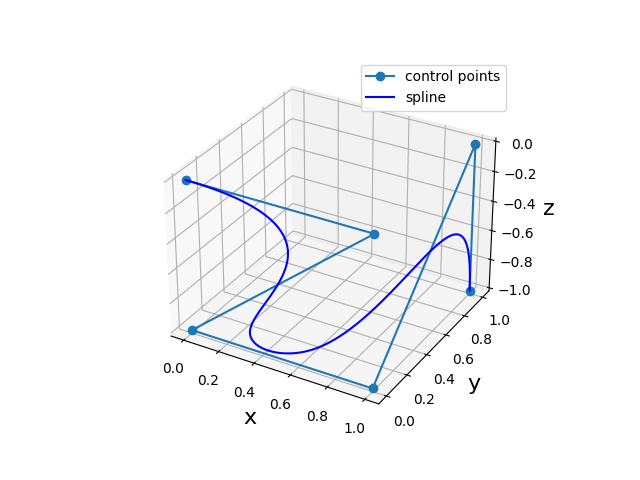
\includegraphics[width=0.5\textwidth]{./figures/example_spline_curve}
  \caption{Example spline curve}
  \label{fig:example_spline_curve}  
\end{figure}

%+++++++++++++++++++++++++++++++
\section{Derivatives of B-splines}

We begin this section by noting that the basis functions and the knot vector do not have to be of the same order.  In fact, if the knot vector has higher order than the basis functions, then the first several basis functions will simply be zero.  
For example, let $\mathbf{t}_3^2 = [0, 0\vdots, 0, 1, 2, 3, \vdots 3, 3]$, then from Equation~\eqref{eq:spline_basis_definition_0} $b_0^0(t; \mathbf{t}_3^2)$, $b_1^0(t; \mathbf{t}_3^2)$, $b_5^0(t; \mathbf{t}_3^2)$, $b_1^0(t; \mathbf{t}_3^2)$, and $b_5^1(t; \mathbf{t}_3^2)$ are equal to zero since the knot intervals in the denominator for those functions are zero.  The remaining basis functions are shown in Figure~\ref{fig:shifting_property}.
\begin{figure}[hbt]
  \centering\includegraphics[width=0.99\textwidth]{./figures/shifting_property}
  \caption{Shifting property of uniform clamped B-spline basis functions.}
  \label{fig:shifting_property}  
\end{figure}
If on the other hand, the knot vector has one order lower, i.e., $\mathbf{t}_3^1 = [0\vdots, 0, 1, 2, 3, \vdots 3]$, then the basis vectors are also shown to the right in Figure~\ref{fig:shifting_property}.  It is clear that reducing the order of the knot vector by one, shifts the index of the basis vectors by one.  We can formalize these observations in the following lemma.
\begin{lemma} \label{lem:shifting_property}
For clamped uniform knot vectors $\mathbf{t}_M^k \in \mathbb{R}^{2k+M+1}$ and $\mathbf{t}_M^{k-1}\in\mathbb{R}^{2k+M-1}$ we have
\[
b_m^j(t; \mathbf{t}_M^k) = b_{m-1}^j(t; \mathbf{t}_M^{k-1}), \qquad j \leq k, \qquad m = 1, \dots, 2k+M.
\]	
Using vector notation we have that
\[
\underbrace{\bbf_M^{k-1}(t; \mathbf{t}_M^{k-1})}_{(M+k-1)\times 1} = S_{M+k} \underbrace{\bbf_M^{k-1}(t; \mathbf{t}_M^k)}_{(M+k)\times 1},
\]
where
\[
	S_{N} \defeq \begin{bmatrix} \mathbf{0}_{(N-1)\times 1}, & \mathbf{I}_{(N-1) \times (N-1)} \end{bmatrix}.
\]
\end{lemma}

We have the following lemma which gives the general formula for the derivative of the spline basis.
\begin{lemma}\label{lem:derivative_basis_functions}
If $\mathbf{t}$ is a general knot vector, then the $0\leq \ell^{th} \leq k$ derivative of the $k^{th}$ order spline function is given by
\[
\frac{d^\ell}{dt^\ell}b_m^k(t; \mathbf{t}) = k\left(\frac{\frac{d^{\ell-1}}{dt^{\ell-1}}b_m^{k-1}(t; \mathbf{t})}{\tau_{m+k}-\tau_m} - \frac{\frac{d^{\ell-1}}{dt^{\ell-1}}b_{m+1}^{k-1}(t; \mathbf{t})}{\tau_{m+k+1}-\tau_{m+1}} \right).
\]	
\end{lemma}
\begin{proof}
See~\cite{PieglTiller95}.
\end{proof}

Using vector notation, we have the following formula for the derivative a spline function.
\begin{lemma} \label{lem:derivative_of_spline}
Given the $k^{th}$-order uniform clamped spline function
\[
\mathbf{p}(t) = \Cbf \bbf_M^k(t), \quad t\in[0, M]
\]
we have that
\[
\frac{d\mathbf{p}}{dt}(t) = \Cbf D_M^k \bbf_M^{k-1}(t), \quad t\in[0, M]
\]	
where $D_M^k$ is the $(M+k)\times (M+k-1)$ derivative matrix of order $k$ given by
\begin{equation}\label{eq:D_k}
D_M^k = -\begin{bmatrix}\bar{D}_M^k \\ \mathbf{0}_{1\times(M+k-1)} \end{bmatrix} + \begin{bmatrix}\mathbf{0}_{1\times(M+k-1)} \\ \bar{D}_M^k \end{bmatrix},
\end{equation}
where
\begin{equation}\label{eq:D_k_bar}
\bar{D}_M^k = \text{diag}\left(\frac{k}{1}, \frac{k}{2}, \dots, \frac{k}{k-1}, \underbrace{1, \dots, 1}_{M-k+1}, \frac{k}{k-1}, \dots, \frac{k}{2}, \frac{k}{1}\right),
\end{equation}
is an $(M+k-1)\times(M+k-1)$ diagonal matrix.
\end{lemma}
\begin{proof}
Noting that
\[
\mathbf{p}(t) = \Cbf \bbf_M^k(t)
              = \sum_{m=0}^{M+k-1} \cbf_m b_m^k(t; \mathbf{t}_M^k),
\]
we have that
\[
\frac{d\mathbf{p}}{dt} = \sum_{m=0}^{M+k-1} \cbf_m \frac{d b_m^k(t; \mathbf{t}_M^k)}{dt}.
\]
From Lemma~\ref{lem:derivative_basis_functions} we get
\begin{align*}
\frac{d\mathbf{p}}{dt} &= \sum_{m=0}^{M+k-1} \cbf_m k\left(\frac{b_m^{k-1}(t; \mathbf{t}_M^k)}{\tau_{m+k}-\tau_m} - \frac{b_{m+1}^{k-1}(t; \mathbf{t}_M^k)}{\tau_{m+k+1}-\tau_{m+1}} \right) \\
&= \sum_{m=0}^{M+k-1} \cbf_m \left[ \left(\frac{k}{\tau_{m+k}-\tau_m}\right) b_m^{k-1}(t; \mathbf{t}_M^k) - \left(\frac{k}{\tau_{m+k+1}-\tau_{m+1}}\right)  b_{m+1}^{k-1}(t; \mathbf{t}_M^k) \right] \\
&= \left(\frac{k}{\tau_{k}-\tau_0}\right)\cbf_0 b_0^{k-1}(t; \mathbf{t}_M^k) + \sum_{m=1}^{M+k-1} \left(\frac{k}{\tau_{m+k}-\tau_m}\right) \left(  \cbf_m - \cbf_{m-1}  \right) b_m^{k-1}(t; \mathbf{t}_M^k) \\
&\qquad - \left(\frac{k}{\tau_{M+2k}-\tau_{M+k}}\right)\cbf_{M+k-1}b_{M+k}^{k-1}(t; \mathbf{t}_M^k).
\end{align*}
Now note that since the first $k+1$ terms in the knot vector $\mathbf{t}_M^k$ are equal to zeros, and the last $k+1$ terms are equal to $M$, that $\tau_k-\tau_0 = \tau_{M+2k}-\tau_{M+k} = 0$, and therefore the first and last terms are zero.  Using the shifting property from Lemma~\ref{lem:shifting_property}, and changing the index by one, we get
\begin{equation}\label{eq:spline_deriviative_1}
\frac{d\mathbf{p}}{dt} = \sum_{m=0}^{M+k-2} \left(\frac{k}{\tau_{m+k}-\tau_{m}}\right) \left( \cbf_{m+1} - \cbf_{m}  \right) b_{m}^{k-1}(t; \mathbf{t}_M^{k-1}),
\end{equation}
where $\tau_\ast$ now corresponds to the knot vector 
\[
\mathbf{t}_M^{k-1} = [\underbrace{0, 0, \dots, 0}_{k-1}, 0, 1, 2, \dots, M, \underbrace{M, \dots, M}_{k-1}].
\]
From the definition of $\mathbf{t}_M^{k-1}$ we note that
\begin{align*}
& \frac{k}{\tau_{k}-\tau_0} = \frac{k}{1}, \quad
\frac{k}{\tau_{k+1}-\tau_1} = \frac{k}{2}, \quad
\dots \quad
\frac{k}{\tau_{2k-1}-\tau_{k-1}} = \frac{k}{k-1},  \\
&\frac{k}{\tau_{2k}-\tau_{k}} = \frac{k}{k}, \quad
\dots \quad
\frac{k}{\tau_{M+k-1} - \tau_{M-1}} = \frac{k}{k}, \\
& \frac{k}{\tau_{M+k} - \tau_{M}} = \frac{k}{k-1}, \quad
\dots \quad
\frac{k}{\tau_{M+2k-2} - \tau_{M+k-2}} = \frac{k}{1}
\end{align*}
Define the $(M+k-1)\times(M+k-1)$ diagonal matrix $\bar{D}_M^k$ in Equation~\eqref{eq:D_k_bar}, and the $(M+k)\times (M+k-1)$ derivative matrix $D_M^k$ in Equation~\eqref{eq:D_k},
then Equation~\eqref{eq:spline_deriviative_1} can be written as
\[
\frac{d\mathbf{p}}{dt} = \Cbf D_M^k \bbf_M^{k-1}(t).
\]
\end{proof}

From Lemma~\ref{lem:derivative_of_spline} we can derive a number of useful results, which we summarize in the corollary below.
\begin{corollary}
	Given the $k^{th}$-order uniform clamped B-spline function
	\[
	\mathbf{p}(t) = \Cbf \bbf_M^k(t), \quad t\in[0, M]
	\]
	we can make the following statements:
	\begin{description}
	\item[(i)] The derivative  $\frac{d\mathbf{p}}{dt}$ is a $(k-1)^{th}$-order uniform clamped B-spline function.
	\item[(ii)] The control points of $\frac{d\mathbf{p}}{dt}$ are given by
		\[
		C^{'} \defeq C D_M^k = \begin{pmatrix}
				\frac{k}{1} (\cbf_1 - \cbf_0)^\top \\
				\vdots \\
				\frac{k}{k-1} (\cbf_{k-1} - \cbf_{k-2})^\top \\
				(\cbf_k - \cbf_{k-1})^\top \\
				\vdots \\
				(\cbf_{M+1} - \cbf_{M})^\top \\
				\frac{k}{k-1} (\cbf_{M+2}-\cbf_{M+1})^\top \\
				\vdots \\
				\frac{k}{1} (\cbf_{M+k-1} - \cbf_{M+k-2})^\top
 				\end{pmatrix}^\top
 			\defeq \begin{pmatrix}
 			        \cbf_0^{'\top} \\
 			        \vdots \\
 			        \cbf_{M+k-2}^{'\top}
 				   \end{pmatrix}^\top.
		\]
	\item[(iii)] The $\ell^{th}$ derivative of $\mathbf{p}(t)$ for $0\leq\ell\leq k-1$ is given by
		\begin{align*}
			\frac{d^{\ell}\mathbf{p}}{dt^{\ell}} 
			&= C D_M^k D_M^{k-1} \dots D_M^{k-\ell+1} \bbf_M^{k-\ell}(t), \quad t\in [0, M] \\
			&= C^{(\ell)} \bbf_M^{k-\ell}(t), \quad t\in [0, M] \\
			&= C \boldsymbol{\psi}^{(\ell)}(t), \quad t\in [0, M] \\
		\end{align*}
		where the control points of the $(k-\ell)^{th}$ order spline are given by
		\[
			C^{(\ell)} = C D_M^k D_M^{k-1} \dots D_M^{k-\ell+1}
		\]
		or alternatively, the $\ell^{th}$ derivative of the basis vector $\bbf_M^k(t)$ is given by
		\[
			\boldsymbol{\psi}^{(\ell)} \defeq \frac{d^{\ell}\bbf_M^k(t)}{dt^{\ell}} = D_M^k D_M^{k-1} \dots D_M^{k-\ell+1} \bbf_M^{k-\ell}(t), \quad t\in [0, M].
		\]
	\item[(iv)] The derivative of $\mathbf{p}(t)$ at $t=0$ is given by the difference of the first two control points as
		\[
			\frac{d\mathbf{p}}{dt}(0) = k(\cbf_1 - \cbf_0).
		\]
	\item[(v)] The derivative of $\mathbf{p}(t)$ at $t=M$ is given by the difference of the last two control points as
		\[
			\frac{d\mathbf{p}}{dt}(M) = k(\cbf_{M+k-1} - \cbf_{M+k-2}).
		\]
	\item[(vi)] If the desired B-spline trajectory with $k\geq 3$ has the following desired endpoint conditions:
		\begin{align*}
			\text{Initial position:} &\quad \mathbf{p}(0) \stackrel{des}{=} \mathbf{p}_0 \\	
			\text{Final position:} &\quad \mathbf{p}(M) \stackrel{des}{=} \mathbf{p}_f \\
			\text{Initial velocity:} &\quad \frac{d\mathbf{p}}{dt}(0) \stackrel{des}{=} \mathbf{v}_0 \\	
			\text{Final velocity:} &\quad \frac{d\mathbf{p}}{dt}(M) \stackrel{des}{=} \mathbf{v}_f, \\
			\text{Initial acceleration:} &\quad \frac{d^2\mathbf{p}}{dt^2}(0) \stackrel{des}{=} \mathbf{a}_0 \\	
			\text{Final acceleration:} &\quad \frac{d^2\mathbf{p}}{dt^2}(M) \stackrel{des}{=} \mathbf{a}_f,
		\end{align*}
		then the first and last three control points satisfy
		\begin{align*}
			\cbf_0 &= \mathbf{p}_0 \\
			\cbf_1 &= \mathbf{p}_0 + \frac{1}{k} \mathbf{v}_0 \\
			\cbf_2 &= \mathbf{p}_0 + \frac{3}{k} \mathbf{v}_0 + \frac{2}{k(k-1)}\mathbf{a}_0 \\
			\cbf_{M+k-3} &= \mathbf{p}_f - \frac{3}{k}\mathbf{v}_f + \frac{2}{k(k-1)}\mathbf{a}_f \\
			\cbf_{M+k-2} &= \mathbf{p}_f - \frac{1}{k}\mathbf{v}_f \\
			\cbf_{M+k-1} &= \mathbf{p}_f.
		\end{align*}
	\end{description}
\end{corollary}


%---------------------------------------------------------------
\section{B-Splines and Solutions of Ordinary Differential Equations}
Given the (single input single output) state space system
\begin{align}
\dot{x} &= Ax + Bu \label{eq:lti-ss-xdot} \\
y &= Cx \label{eq:lti-ss-y}
\end{align}
with initial condition $x(t_0)=x_0$, the solution to the differential equation at time $t\geq t_0$ is given by
\[
y(t) = Ce^{A(t-t_0)}x_0 + \int_{t_0}^t Ce^{A(t-\tau)} B u(\tau) \, d\tau.
\]
Suppose that the input is given by the spline function
\[
u(t) = \sum_{j=0}^{n-1} c_j \phi_j(t) \defeq \cbf^\top \boldsymbol{\phi}(t),
\]
then the solution to the differential equation is given by
\begin{align*}
	y(t) &= Ce^{A(t-t_0)}x_0 + \int_{t_0}^t Ce^{A(t-\tau)} B \left(\sum_{j=0}^{n-1} c_j \phi_j(\tau)\right) \, d\tau \\
	     &= Ce^{A(t-t_0)}x_0 + \sum_{j=0}^{n-1} c_j \left(\int_{t_0}^t Ce^{A(t-\tau)} B \phi_j(\tau)\, d\tau \right).
\end{align*}
Defining the function
\[
\psi_j(t) \defeq \int_{t_0}^t Ce^{A(t-\tau)} B \phi_j(\tau)\, d\tau
\]
and the vector $\boldsymbol{\psi}(t) = (\psi_0(t), \dots, \psi_{n-1}(t))^\top$, then
\begin{equation} \label{eq:lti-ss-soln}
y(t) = Ce^{A(t-t_0)}x_0 + \cbf^\top \boldsymbol{\psi}(t).
\end{equation}

Using this framework, we can solve a variety of open-loop control problem.
\begin{example}
Given the dynamic system represented by Equations~\eqref{eq:lti-ss-xdot}--\eqref{eq:lti-ss-y}, find $u(t)$ to transfer the system from $y_0=Cx_0$, to a desired final output $y(t_f)=y_f$.  From Equation~\eqref{eq:lti-ss-soln} we have
\[
y_f = Ce^{A(t_f-t_0)}x_0 + \boldsymbol{\psi}(t_f)^\top \cbf.
\]
If we assume that $\cbf = \zeta \boldsymbol{\psi}(t_f)$, where $\zeta\in\mathbb{R}$, then $\zeta$ satisfies
\begin{align*}
	& y_f - Ce^{A(t_f-t_0)}x_0 = \boldsymbol{\psi}(t_f)^\top \boldsymbol{\psi}(t_f) \zeta \\
	\implies & \zeta = \frac{y_f - Ce^{A(t_f-t_0)}x_0}{\norm{\boldsymbol{\psi}(t_f)}^2}.
\end{align*}
Therefore, the spline coefficients that transfer the system between the two desired outputs are
\[
\cbf = \left(\frac{\boldsymbol{\psi}(t_f)}{\norm{\boldsymbol{\psi}(t_f)}^2}\right) \left(y_f - Ce^{A(t_f-t_0)}x_0 \right).
\]
\end{example}

\begin{example}
	Assume that the initial condition is $x_0$, and assume that the control objective is to follow a reference signal $y_r(t)$.    
	Find the control signal that minimizes the integral of the squared error:
	\begin{equation} \label{eq:example_min_tracking_norm}
	\int_0^{t_f} \norm{y(\tau) - y_r(\tau)}^2 d\tau.
	\end{equation}
	In this case we have
	\begin{align*}
			\int_0^{t_f} \norm{y(\tau) - y_r(\tau)}^2 d\tau 
				&= \int_0^{t_f} (y(\tau) - y_r(\tau))^\top (y(\tau)-y_r(\tau)) d\tau \\
				&= \int_0^{t_f} (\boldsymbol{\psi}(\tau)^\top \cbf  - y_r(\tau))^\top (\boldsymbol{\psi}(\tau)^\top \cbf-y_r(\tau)) d\tau \\
				&= \int_0^{t_f} \left(\cbf^\top \boldsymbol{\psi}(\tau) \boldsymbol{\psi}(\tau)^\top \cbf
					 - 2 y_r(\tau) \boldsymbol{\psi}(\tau)^\top \cbf + \norm{y_r(\tau)}^2 \right) d\tau \\
				&= \cbf^\top \left(\int_0^{t_f} \boldsymbol{\psi}(\tau) \boldsymbol{\psi}(\tau)^\top d\tau \right) \cbf
					 - 2 \left(\int_0^{t_f} y_r(\tau) \boldsymbol{\psi}(\tau)^\top d\tau\right) \cbf 
					 \\ &\qquad
					 + \left(\int_0^{t_f}\norm{y_r(\tau)}^2  d\tau \right) \\
				&= \cbf^\top A \cbf - 2 b^\top \cbf + d
	\end{align*}
	where
	\begin{align*}
		A &= \int_0^{t_f} \boldsymbol{\psi}(\tau) \boldsymbol{\psi}(\tau)^\top d\tau \\
		b &= \int_0^{t_f} y_r(\tau) \boldsymbol{\psi}(\tau) d\tau \\
		d &= \int_0^{t_f}\norm{y_r(\tau)}^2  d\tau.
	\end{align*}
	
	The (unconstrained) control input that minimizes Equation~\eqref{eq:example_min_tracking_norm} satisfies
	\[
	2 A \cbf - 2 b = 0.
	\]
	Therefore, the spline coefficients are given by
	\[
	\cbf = A^{-1}b = \left(\int_0^{t_f} \boldsymbol{\psi}(\tau) \boldsymbol{\psi}(\tau)^\top d\tau \right)^{-1} \left(\int_0^{t_f} y_r(\tau) \boldsymbol{\psi}(\tau) d\tau \right).
	\]5
\end{example}






%---------------------------------------------------------------
\section{B-Spline Planning for Chains of Integrators}

%---------------------------------------------------------------
\section{B-Splines on Lie Groups}

%---------------------------------------------------------------
\section{B-Splines Surfaces}

Suppose that the objective is to create a one dimensional surface over a two dimensional domain.  For example, a terrain map is a one dimensional surface of altitudes over the north-east plane.  In this section we will explore the use of B-splines to accomplish this objective. Many of the ideas and notation in this section come from~\cite{RodriguesTsiogkasAguiar20}.

If $\mathbf{t}_M^k$ and $\mathbf{t}_N^k$ are two different $k^{th}$ order uniform clamped knot vectors of length $M$ and $N$ understood to define knots in the $x$ and $y$ directions, then following Equation~\eqref{eq:clamped_uniform_spline}, a clamped uniform B-spline surface is defined as 
\begin{equation}\label{eq:spline_surface1}
S(x, y) \defeq \sum_{m=0}^{M+k-1} \sum_{n=0}^{N+k-1} c_{m,n} b^k_m(x; \mathbf{t}_M^k) b^k_n(y; \mathbf{t}_N^k), \quad x\in[0,M], y\in[0, N],
\end{equation}
where $c_{m, n}$, $m=0, \dots, M+k-1$, $n=0, \dots, N+k-1$ are the control points of the surface.  Defining the matrix $\Cbf=\{c_{m,n}\}$, and defining the spatial variable $\sbf = (s_1, s_2)^\top$, we can write Equation~\eqref{eq:spline_surface1} as
\begin{equation}\label{eq:spline_surface2}
S(\sbf) = \bbf^k_M(s_1)^\top \Cbf \bbf^k_N(s_2), \quad \sbf\in[0, M]\times[0, N],
\end{equation}
This equation is linear in the spline coefficients $\Cbf$.  In other words, if $S_1(\sbf)=\bbf^k_M(s_1)^\top \Cbf_1 \bbf^k_N(s_2)$, and $S_1(\sbf)=\bbf^k_M(s_1)^\top \Cbf_2 \bbf^k_N(s_2)$ are two different spline surfaces, then 
\[
S(\sbf)\defeq \alpha S_1(\sbf) + \beta S_2(\sbf) = \bbf^k_M(s_1)^\top \left(\alpha\Cbf_1 + \beta\Cbf_2\right) \bbf^k_N(s_2),
\]
is also a spline surface.

Suppose that instead of defining the surface over the set $[0, M]\times[0, N]$ we instead would like to define the surface over the set $[\underline{X}, \overline{X}]\times[\underline{Y}, \overline{Y}]$.  Given the shift and scaling properties is Lemmas~\ref{lem:basis_are_shift_invariant} and~\ref{lem:bases_are_scale_invariant} we have 
\begin{equation}\label{eq:spline_surface3}
S(\sbf) = \bbf^k_M\left(\frac{M(s_1-\underline{X})}{\overline{X}-\underline{X}}\right)^\top \Cbf \bbf^k_N\left(\frac{N(s_2-\underline{Y})}{\overline{Y}-\underline{Y}}\right), \quad \sbf\in[\underline{X}, \overline{X}]\times[\underline{Y}, \overline{Y}].
\end{equation}

\begin{figure}[hbt]
  \centering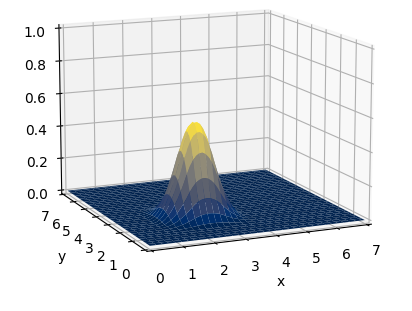
\includegraphics[width=0.9\textwidth]{./figures/spline_surface_basis}
  \caption{A single second order spline bases function $b_3^2(s_1)b_3^2(s_2)$.}
  \label{fig:spline_surface_bases}  
\end{figure}


%
%The basic idea is to create two-dimensional bases vectors as the tensor product of the one-dimensional bases vectors introduced in Section~\ref{sec:b-spline-basis-functions}.  For example, replacing the time variable $t$ with the spacial variables $x$ and $y$, the $k^{th}$-order two dimensional basis vectors are defined as
%\[
%b^k_{m,n}(x,y) = b^k_m(x; \mathbf{t}_1) b^k_n(y; \mathbf{t}_2), 
%\]
%where $T=\mathbf{t}_1 \times \mathbf{t}_2$ is the two-dimensional knot array, and $b^{k}_m(x; \mathbf{t}_1)$ is the $k^{th}$-order spline function with index $m$ and knot vector $\mathbf{t}_1$, and similarly for $b^k_n(y; \mathbf{t}_2)$.
%
%
%If $\mathbf{t}_M^k$ and $\sbf_N^k$ are $k^{th}$ order uniform clamped knot vectors of length $M$ and $N$, then 
%$\mathbf{T}^k_{M,N}\defeq \mathbf{t}_M^k \times \sbf_M^k$ is a $k^{th}$ order uniform clamped knot array of size (M,N).  For example, if $\mathbf{t}_3^2 = [0, 0, 0, 1, 2, 3, 3, 3]$, and $\sbf_2^2 = [0, 0, 0, 1, 2, 2, 2]$, then
%\[
%\mathbf{T}^2_{3,2} = \begin{bmatrix} 
%						(0, 0) & (0, 0) & (0, 0) & (0, 1) & (0, 2) & (0, 2) & (0, 2) \\
%						(0, 0) & (0, 0) & (0, 0) & (0, 1) & (0, 2) & (0, 2) & (0, 2) \\
%						(0, 0) & (0, 0) & (0, 0) & (0, 1) & (0, 2) & (0, 2) & (0, 2) \\
%						(1, 0) & (1, 0) & (1, 0) & (1, 1) & (1, 2) & (1, 2) & (1, 2) \\
%						(2, 0) & (2, 0) & (2, 0) & (2, 1) & (2, 2) & (2, 2) & (2, 2) \\
%						(3, 0) & (3, 0) & (3, 0) & (3, 1) & (2, 2) & (3, 2) & (3, 2) \\
%						(3, 0) & (3, 0) & (3, 0) & (3, 1) & (2, 2) & (3, 2) & (3, 2) \\
%						(3, 0) & (3, 0) & (3, 0) & (3, 1) & (2, 2) & (3, 2) & (3, 2)
% 					 \end{bmatrix}.
%\]
%
%
%Recall that if $\mathbf{A}$ is an $m\times n$ matrix and $\bbf$ is $p\times q$ matrix, then the Kronecker product of $\mathbf{A}$ and $\bbf$ is defined as 
%\[
%\mathbf{A}\otimes\bbf \circeq \begin{pmatrix} 
% 										a_{11}B & a_{12}B & \dots & a_{1n}B \\	
% 										a_{21}B & a_{22}B & \dots & a_{2n}B \\
% 										\vdots & \vdots & \dots & \vdots \\
% 										a_{m1}B & a_{m2}B & \dots & a_{mn}B \\	
% 									\end{pmatrix}.
%\]
%We will use the Kronecker product to simplify the notation associated with spline surfaces.  Let $\xbf=(x_1, x_2)^\top\in\mathbb{R}^2$, and let $\bbf^k_M(x_1; \mathbf{t}_M^k)$ and $\bbf^k_N(x_2; \sbf_N^k$ be $k^{th}$ order basis vectors as defined in Equation~\eqref{eq:basis_vector} and $T^k_{M,N}=\mathbf{t}_M^k \times \sbf_N^k$, then define the basis vector 
%\[
%\bbf^k_{M,N}(\xbf; T^k_{M,N}) = \bbf^k_M(x_1; \mathbf{t}_M^k) \otimes \bbf^k_N(x_2; \sbf_N^k), 
%\]
%where we will drop to inclusion of the knot array and write simply $\bbf^k_{M,N}(\xbf)\circeq\bbf^k_{M,N}(\xbf; T^k_{M,N})$.
%Similarly, defining the control vector 
%\[
%\cbf \circeq \begin{pmatrix} c_{1,1} & c_{1,2} & \dots & c_{1,N} & \dots & c{M,1} & \dots & c_{M,N} \end{pmatrix}^\top,
%\]
%we get that
%\[
%S^k(\xbf) = \cbf^\top  \bbf^k_{M,N}(\xbf), \qquad \xbf \in [0,M]\times[0,N].
%\]

The Python code below plots a randomly defined terrain map over the domain $[-\pi, \pi]\times[-2\pi, 2\pi]$.
\begin{lstlisting}
import numpy as np
import splipy as sp
import matplotlib.pyplot as plt
from bspline_tools import uniform_clamped_knots

def draw_random_surface(order=2, M=10, N=10,
                        Xmin=-3.14159, Xmax=3.14159,
                        Ymin=-2*3.14159, Ymax=2*3.14159):
    # define the spline surface
    knots_x = uniform_clamped_knots(k=order, M=M)
    knots_y = uniform_clamped_knots(k=order, M=N)
    basis_x = sp.BSplineBasis(order + 1, knots_x)
    basis_y = sp.BSplineBasis(order + 1, knots_y)
    C = np.random.rand(M + order, N + order)  # random control points
    surface = sp.Surface(basis_x, basis_y,
                         np.reshape(C, ((M + order) * (N + order), 1)))
    # plot the spline surface
    x = np.linspace(Xmin, Xmax, 10 * M)
    y = np.linspace(Ymin, Ymax, 10 * N)
    S = surface(M*(x-Xmin)/(Xmax-Xmin),
                N*(y-Ymin)/(Ymax-Ymin))  # surface points
    fig = plt.figure()
    ax = fig.add_subplot(111, projection='3d')
    plt.xlabel('x')
    plt.ylabel('y')
    x_pts, y_pts = np.meshgrid(x, y)  # grid points
    ax.plot_surface(x_pts, y_pts, S[:, :, 0])
    plt.show()
\end{lstlisting}
The result of running this code is shown in Figure~\ref{fig:random_spline_surface}
\begin{figure}[hbt]
  \centering\includegraphics[width=0.9\textwidth]{./figures/random_spline_surface}
  \caption{Spline surface with randomly generated control points.}
  \label{fig:random_spline_surface}  
\end{figure}





%---------------------------------------------------------------
\section{B-Splines and Occupancy Maps}

Since B-spline surfaces are continuous the spatial variable $\sbf\in\mathbf{R}^2$, the occupancy map will also be continuous (as opposed to an occupancy grid).  Following~\cite{RodriguesTsiogkasAguiar20}, at every point $\sbf$ we can define the discrete random variable $m(\sbf)$ to be the occupancy of the map, where $m(\sbf)=1$ indicates that a target is located at $\sbf$, and $m(\sbf)=0$ indicates that a target is not located at $\sbf$.  
%
Similarly, define the discrete random variable $z(\sbf)$ to be the measurement state, where $z(\sbf)=1$ indicates that a target is detected at $\sbf$, and $z(\sbf)=0$ indicates that a target is not detected at $\sbf$.
% 
Let $\xbf_t$ be the state of the UAV at time $t$, where the UAV state evolution equations are given by
\[
\xbf_t = f(\xbf_{t-1}, \ubf_{t-1}) + \eta_t
\]
where $\eta_t\sim\mathcal{N}(0, Q)$. Let $\fov{\xbf_t}$ be the area on the terrain what is seen by the camera when the state is $\xbf_t$, then the measurement model is given by
%
\begin{align}
	p(z(\sbf)=1 \mid m(\sbf)=1, \xbf) &= \begin{cases}
 											p_d &\quad \mathbf{s}\in\fov{\xbf} \\
 											0 &\quad \text{otherwise}
 										 \end{cases} 
	\label{eq:prob_z=1:m=1}\\
	p(z(\sbf)=0 \mid m(\sbf)=1, \xbf) &= \begin{cases}
 											1-p_d &\quad \mathbf{s}\in\fov{\xbf} \\
 											1 &\quad \text{otherwise}
 										 \end{cases}
	\label{eq:prob_z=0:m=1}\\
	p(z(\sbf)=1 \mid m(\sbf)=0, \xbf) &= \begin{cases}
 											p_f &\quad \mathbf{s}\in\fov{\xbf} \\
 											1 &\quad \text{otherwise}
 										  \end{cases}
	\label{eq:prob_z=1:m=0}\\
	p(z(\sbf)=0 \mid m(\sbf)=0, \xbf) &= \begin{cases}
 											1-p_f &\quad \mathbf{s}\in\fov{\xbf} \\
 											0 &\quad \text{otherwise}
 										  \end{cases},
 	\label{eq:prob_z=1:m=0}
\end{align}
where $p_d$ is the probability of detection, and $p_f$ is the probability of false alarm.

Let $Z_t(\sbf) = \{z_t(\sbf), z_{t-1}(\sbf), \dots, z_0(\sbf)\}$ be the set of measurements of map location $\sbf$ over the time horizon $[0, t]$.  Using Bayes's law we have
\begin{align*}
	p(m(\sbf)=1 \mid Z_t(\sbf)) &= \frac{p(z_t(\sbf)\mid m(\sbf)=1, Z_{t-1}(\sbf)) p(m(\sbf)=1 \mid Z_{t-1}(\sbf))}{p(z_t(\sbf) \mid Z_{t-1}(\sbf))} \\
	p(m(\sbf)=0 \mid Z_t(\sbf)) &= \frac{p(z_t(\sbf)\mid m(\sbf)=0, Z_{t-1}(\sbf)) p(m(\sbf)=0 \mid Z_{t-1}(\sbf))}{p(z_t(\sbf) \mid Z_{t-1}(\sbf))}
\end{align*}
Defining the odds of a discrete random variable as
\[
\odd{x} \defeq \frac{p(x=1)}{p(x=0)},
\]
we get that 
\begin{align*}
	\odd{m(\sbf)\mid Z_t(\sbf), \xbf_t} &= \frac{p(m(\sbf)=1 \mid Z_t(\sbf), \xbf_t)}{p(m(\sbf)=0 \mid Z_t(\sbf), \xbf_t)} \\
	&= \frac{p(z_t(\sbf) \mid m(\sbf)=1, Z_{t-1}(\sbf), \xbf_t) \, p(m(\sbf)=1)\mid Z_{t-1}(\sbf), \xbf_t)}{p(z_t(\sbf)\mid m(\sbf)=0, Z_{t-1}(\sbf), \xbf_t) \, p(m(\sbf)=0)\mid Z_{t-1}(\sbf), \xbf_t)} \\
	&= \odd{m(\sbf) \mid Z_{t-1}(\sbf), \xbf_t}  \frac{p(z_t(\sbf)\mid m(\sbf)=1, Z_{t-1}(\sbf), \xbf_t)}{p(z_t(\sbf)\mid m(\sbf)=0, Z_{t-1}(\sbf), \xbf_t)}.
\end{align*}
Assuming that the current measurement is conditionally independent of previous measurements we get
\begin{align*}
	\odd{m(\sbf)\mid Z_t(\sbf), \xbf_t} 
		&= \odd{m(\sbf) \mid Z_{t-1}(\sbf), \xbf_t}  \frac{p(z_t(\sbf)\mid m(\sbf)=1, \xbf_t)}{p(z_t(\sbf)\mid m(\sbf)=0, \xbf_t)}.
\end{align*}
Taking the natural logarithm of each side gives
\[
\log\odd{m(\sbf)\mid Z_t(\sbf), \xbf_t} = \log \odd{m(\sbf) \mid Z_{t-1}(\sbf), \xbf_t} + \log\left(\frac{p(z_t(\sbf)\mid m(\sbf)=1, \xbf_t)}{p(z_t(\sbf)\mid m(\sbf)=0, \xbf_t)}\right).
\]
Defining the expected value (over random variable $\xbf_t$) as
\[
S_t(\sbf) \defeq E\{\log\odd{m(\sbf)\mid Z_t(\sbf), \xbf_t}\},
\]
then the expected log-odds surface at time $t$ is given by
\[
S_t(\sbf) = S_{t-1}(\sbf) + \int\log\left[ \frac{p(z_t(\sbf)\mid m(\sbf)=1, \xbf_t)}{p(z_t(\sbf)\mid m(\sbf)=0, \xbf_t)}\right]p(\xbf_t)d\xbf_t.
\] 

Defining the measurement function as 
\begin{equation} \label{eq:measurement_function}
U(z_t(\sbf), \sbf) \defeq \int\log\left[ \frac{p(z_t(\sbf)\mid m(\sbf)=1, \xbf_t)}{p(z_t(\sbf)\mid m(\sbf)=0, \xbf_t)}\right]p(\xbf_t)d\xbf_t,	
\end{equation}
then the log-odds update expression is
\begin{equation}\label{eq:log_odds_surface_update}
S_t(\sbf) = S_{t-1}(\sbf) + U(z_t(\sbf), \sbf).
\end{equation}

Following~\cite{RodriguesTsiogkasAguiar20} we will represent $S_t(\sbf)$ using a B-spline surface as 
\begin{equation}\label{eq:log_odds_surface}
S_t(\sbf) = \bbf_M^k(s_1)^\top C_t \bbf_N^k(s_2), \quad \sbf \in [0,M]\times[0,N].
\end{equation}
The probability that the target is located at $\sbf$ can be recovered from $S_t(\sbf)$ using the formula
\[
p(m(\sbf)=1\mid Z_t(\sbf)) = \frac{e^{S_t(\sbf)}}{1+e^{S_t(\sbf)}}.
\]

\begin{lemma}\label{lem:measurement_update_equation}
	Given the log-odds spline surface~\eqref{eq:log_odds_surface}, a measurement function $U(z_t(\sbf), \sbf)$, and the log-odds update equation~\eqref{eq:log_odds_surface_update}, the optimal update for the spline coefficients after a measurement at $\sbf \in [0,M]\times[0,N]$ is given by
	\begin{equation}\label{eq:coefficient_update_3}
	\Cbf_t = \Cbf_{t-1} + \mathbf{B}_{M,N}^k(\sbf) U(z_t(\sbf), \sbf), 
	\end{equation}
	where
	\begin{equation}\label{eq:measurement_update_matrix_B}
	\mathbf{B}_{M,N}^k(\sbf) \defeq \frac{\bbf_M^k(s_1)\bbf_N^k(s_2)^\top}{\norm{\bbf_M^k(s_1)}^2\norm{\bbf_N^k(s_2)}^2}
	\end{equation}
\end{lemma}
\begin{proof}
The proof follows the discussion given in~\cite[Section III.A]{RodriguesTsiogkasAguiar20}.
%
Define the $\vec{\cdot}$ operation on a matrix to be the operation of stacking all of the columns of a matrix into a single vector, i.e., $\vec{(\cbf_1, \dots, \cbf_N)}=(\cbf_1^\top, \dots, \cbf_N^\top)^\top$, and let $\otimes$ denote the Kronecker product. As shown in~\cite{Kronecker_vect}, if $A$, $X$, and $B$ are compatible matrices, then $\vec{AXB}=(B^\top \otimes A)\vec{X}$.  Accordingly, we can write the spline surface~\eqref{eq:log_odds_surface} as
\begin{align*}
S_t(\sbf) &= \bbf_M^k(s_1)^\top \Cbf_t \bbf_N^k(s_2) \\
		  &= \vec{\bbf_M^k(s_1)^\top \Cbf_t \bbf_N^k(s_2)} \\
		  &= \left[\bbf_N^k(s_2)^\top \otimes \bbf_M^k(s_1)^\top \right] \vec{\Cbf_t} \\
		  &= \phibf(\sbf)^\top \cbf_t,
\end{align*}
where $\phibf(\sbf)\defeq \bbf_N^k(s_2) \otimes \bbf_M^k(s_1)$, and $\cbf_t \defeq \vec{\Cbf_t}$.

Consider the log-odds update Equation~\eqref{eq:log_odds_surface_update}, define the error equation at $\sbf$ to be
\begin{equation}\label{eq:error_log_odds}
e(\cbf_t) \defeq \phibf(\sbf)^\top \cbf_t - \phibf(\sbf)^\top \cbf_{t-1} - U(z_t(\sbf), \sbf),
\end{equation}
and consider the cost function $J(\cbf_t)=\frac{1}{2}e(\cbf_t)^2$.  Using a gradient descent update law for $\cbf_t$ would result in
\begin{align*}
\cbf_t &= \cbf_{t-1} - \mu \frac{\partial J}{\partial\cbf_t} \\
       &= \cbf_{t-1} - \mu \frac{\partial e}{\partial\cbf_t} e(\cbf_t) \\
	   &= \cbf_{t-1} - \mu \phibf(\sbf) e(\cbf_t) \\
	   &= \cbf_{t-1} - \mu \phibf(\sbf) \left(\phibf(\sbf)^\top \cbf_t - \phibf(\sbf)^\top \cbf_{t-1} - U(z_t(\sbf), \sbf)\right).
\end{align*}
Solving for $\cbf_t$ gives 
\begin{equation}\label{eq:coefficient_update_1}
\cbf_t = \cbf_{t-1} + \mu \left[I + \mu \phibf(\sbf)\phibf(\sbf)^\top\right]^{-1}\phibf(\sbf) U(z_t(\sbf), \sbf),
\end{equation}
where we note that $\left[I + \mu \phibf(\sbf)\phibf(\sbf)^\top\right]$ is invertible for all $\mu>0$ since $\phibf\phibf^\top$ is positive semi-definite.  From the matrix inversion lemma we have that
\[
\left[I + \mu \phibf(\sbf)\phibf(\sbf)^\top\right]^{-1} = I - \mu\frac{\phibf(\sbf)\phibf(\sbf)^\top}{1+\mu\norm{\phibf(\sbf)}^2}.
\]
Therefore Equation~\eqref{eq:coefficient_update_1} becomes
\begin{align}
	\cbf_t &= \cbf_{t-1} + \mu \left[I - \mu\frac{\phibf(\sbf)\phibf(\sbf)^\top}{1+\mu\norm{\phibf(\sbf)}^2}\right]\phibf(\sbf)		   U(z_t(\sbf), \sbf) \notag \\
	       &= \cbf_{t-1} + \mu \phibf(\sbf)\left[1 - \mu\frac{\norm{\phibf(\sbf)}^2}{1+\mu\norm{\phibf(\sbf)}^2}\right]U(z_t(\sbf), \sbf) \notag \\
	       &= \cbf_{t-1} + \left[\frac{\mu}{1+\mu\norm{\phibf(\sbf)}^2}\right]\phibf(\sbf) U(z_t(\sbf), \sbf).
	       \label{eq:coefficient_update_2}
\end{align}
The error equation~\eqref{eq:error_log_odds} then becomes
\[
e(\cbf_t) = \left[\frac{\mu\norm{\phibf(\sbf)}^2}{1+\mu\norm{\phibf(\sbf)}^2}\right] U(z_t(\sbf), \sbf) - U(z_t(\sbf), \sbf).
\]
Therefore, the squared error is minimized in the limit as $\mu\to\infty$.  As $\mu\to\infty$, the spline coefficient update equation~\eqref{eq:coefficient_update_2} becomes
\[
\cbf_t = \cbf_{t-1} + \frac{\phibf(\sbf)}{\norm{\phibf(\sbf)}^2} U(z_t(\sbf), \sbf),
\]
or in other words
\[
\vec{\Cbf_t} = \vec{\Cbf_{t-1}} + \frac{\bbf_N^k(s_2) \otimes \bbf_M^k(s_1)}{\norm{\bbf_N^k(s_2) \otimes \bbf_M^k(s_1)}^2} U(z_t(\sbf), \sbf).
\]
Unstacking the vectors into matrices, and noting that 
\[
\bbf_N^k(s_2) \otimes \bbf_M^k(s_1)=\vec{\bbf_M^k(s_1)\bbf_N^k(s_2)^\top}
\]
and that 
\[
\norm{\bbf_N^k(s_2) \otimes \bbf_M^k(s_1)}^2=\norm{\bbf_M^k(s_1)}^2 \norm{\bbf_N^k(s_2)}^2,
\] 
results in Equation~\eqref{eq:coefficient_update_3}.
\end{proof}

\begin{lemma} \label{lem:B_is_sparse}
Let $\mathbf{B}_{M,N}^k(\sbf)$
be the $(M+k)\times(N+k)$ measurement update matrix defined in Equation~\eqref{eq:measurement_update_matrix_B}.  
If $\sbf \in [m, m+1]\times[n, n+1] \subset [0, M]\times[0,N]$, then the only nonzero elements of $\mathbf{B}_{M,N}^k(\sbf)$ is the $(k+1)\times(k+1)$ sub-matrix with upper-left index equal to $[m,n]$.
\end{lemma}
\begin{proof}
The proof follows directly from Lemma~\ref{lem:finite_num_control_points}.	
\end{proof}

Lemma's~\ref{lem:measurement_update_equation} and~\ref{lem:B_is_sparse} taken together imply that every measurement $U(z_t(\sbf), \sbf)$ only requires the update of $(k+1)^2$ spline coefficients, and is therefore, extremely computationally efficient.  For example, if the order of the splines is $k=3$, then the measurement update is over a $4\times 4$ submatrix, independent of the size of $M$ and $N$, which for large worlds could be in tens of thousands.  This property has obvious implications for cooperative control where vehicles can build cooperative maps with limited communication.  


We now turn our attention to the computation of the update equation $U(z_t(\sbf), \sbf)$ given by Equation~\eqref{eq:measurement_function} as
\[
U(z_t(\sbf), \sbf) = \int_{\xibf\in\mathbb{R}^n}\log\left[ \frac{p(z_t(\sbf)\mid m(\sbf)=1, \xbf_t)}{p(z_t(\sbf)\mid m(\sbf)=0, \xbf_t)}\right]p_{X_t}(\xibf)d\xibf,
\]
where 
\[
p_{X_t}(\xibf) \defeq \frac{1}{\sqrt{2\pi^n|P_t|}}exp\left(\frac{1}{2}(\xibf-\xbf_t)^\top \Pbf_t^{-1} (\xibf-\xbf_t)\right)
\]
is the posterior probability density associated with state estimate of the aircraft, where $(\xbf_t, \Pbf_t)$ are the mean and covariance given by, for example, an extended Kalman filter.
From Equations~\eqref{eq:prob_z=1:m=1}--\eqref{eq:prob_z=1:m=0} we get that 
\[
\log\left[ \frac{p(z_t(\sbf)\mid m(\sbf)=1, \xbf_t)}{p(z_t(\sbf)\mid m(\sbf)=0, \xbf_t)}\right] 
	= \begin{cases}
 		\log\left(\frac{p_d}{p_f}\right), &\quad z_t(\sbf)=1 \text{~and~} \sbf\in\fov{\xbf_t} \\
 		\log\left(\frac{1-p_d}{1-p_f}\right), &\quad z_t(\sbf)=0 \text{~and~} \sbf\in\fov{\xbf_t} \\
 		? &\quad \sbf\not\in\fov{\xbf_t}
 	  \end{cases}.
\]
Defining the set $\fovinv{\sbf}\defeq\{\xibf\in\mathbb{R}^n: \sbf\in\fov{\xibf}\}$ and defining 
\begin{equation}\label{eq:Ubar}
\bar{U}(\sbf) \defeq \int_{\xibf\in\fovinv{\sbf}} p_{X_t}(\xibf)d\xibf
\end{equation}
we get that the measurement update equation is given by
\[
U(z_t(\sbf), \sbf) = 
	\begin{cases}
 		\bar{U}(\sbf)\log\left(\frac{p_d}{p_f}\right), &\quad z_t(\sbf)=1 \\
 		\bar{U}(\sbf)\log\left(\frac{1-p_d}{1-p_f}\right), &\quad z_t(\sbf)=0
 	  \end{cases}.
\]

The computation of $\bar{U}(\sbf)$ will require a few assumptions, as well as numerical approximation of the integral.
In approximating Equation~\eqref{eq:Ubar} we will assume that the field of view of the camera is rectangular with field-of-view angles $\eta_x$, and $\eta_y$ in the $x$ and $y$ axes of the camera frame. 
%
\begin{figure}[hbt]
  \centering\includegraphics[width=0.99\textwidth]{./figures/inverse_field_of_view}
  \caption{Field-of-view of the camera given $\xbf_t$, and inverse field-of-view of the camera given $\sbf$.}
  \label{fig:inverse_field_of_view}  
\end{figure}
%
Figure~\ref{fig:inverse_field_of_view} shows the physical geometry.  We will assume that the camera is gimbaled to point toward the center of the earth, and that the ground is approximately flat.  In that case, the physical footprint of the camera field of view will also be rectangular with physical dimensions given by $M_x = 2h\tan(\eta_x/2)$ and $M_y=2h\tan(\eta_y/2)$, where $h=-p_d$ is the altitude of the aircraft.  For the purposes of this section, we will assume that there is uncertainty in the north-east position of the aircraft, but that the altitude and attitude are known.  If the aircraft is equipped with an altimeter and digital compass, then this is a reasonable assumption.  
Given the estimated state of the UAV $\xbf_t$ we can determine footprint of field-of-view on the ground.  We assume that the target detection software can detect targets to some resolution in the camera, and divide the field of view into rectangular bins accordingly.  Define $N_x$ and $N_y$ so that there are $2N_x+1$ bins in the $x$-direction, and $2N_y+1$ bins in the $y$-direction, as shown in Figure~\ref{fig:riemann_sum}.  We define the number of bins in this way to ensure an odd number in each direction. 
\begin{figure}[hbt]
  \centering\includegraphics[width=0.99\textwidth]{./figures/riemann_sum}
  \caption{Riemann sum over camera field-of-view.}
  \label{fig:riemann_sum}  
\end{figure}
The physical size of each bin is given by
\[
	A = \left(\frac{M_x}{2N_x+1}\right)\left(\frac{M_y}{2N_y+1}\right)
	  = \left(\frac{2h\tan(\eta_x/2)}{2N_x+1}\right)\left(\frac{2h\tan(\eta_y/2)}{2N_y+1}\right).
\]

Suppose that the state of the UAV at time $t$ is given by
\[
\xbf_t = (p_n, p_e, p_d, v_n, v_e, v_d, \phi, \theta, \psi)^\top
\]
then the position of the center of the $(i,j)^{th}$ bin is given by
\[
\sbf_{i,j} = \begin{pmatrix} p_n \\ p_e \end{pmatrix} + \begin{pmatrix} 0 & -1 \\ 1 & 0 \end{pmatrix} \begin{pmatrix}\cos\psi & \sin\psi \\ -\sin\psi & \cos\psi \end{pmatrix}\begin{pmatrix} \frac{M_x(h)}{2N_x+1} i \\ \frac{M_y(h)}{2N_y+1} j \end{pmatrix}, 
\]
for $i=-N_x, \dots, N_x$ and $j=-N_y, \dots, N_y$.  

Given a camera measurement, we will need to update the log-odds spline map for each $\sbf_{i,j}$ in the camera field of view. To compute $\bar{U}(\sbf_{i,j})$ requires the inverse field-of-view of $\sbf_{i,j}$.  Under the assumption that the $h$ and $\psi$ are known, the inverse field-of-view will a rectangle on the altitude plane of the aircraft centered at $\sbf_{i,j}$ as shown in Figure~\ref{fig:inverse_field_of_view}.  Using a similar binning notation for the inverse field-of-view, the north-east coordinates of the center of the $(m,n)^{th}$ bin of the inverse field of view is given by
\begin{align*}
&\sbf_{i,j} + \begin{pmatrix} 0 & -1 \\ 1 & 0 \end{pmatrix} \begin{pmatrix}\cos\psi & \sin\psi \\ -\sin\psi & \cos\psi \end{pmatrix}\begin{pmatrix} \frac{M_x(h)}{2N_x+1} m \\ \frac{M_y(h)}{2N_y+1} n \end{pmatrix} \\
=& \begin{pmatrix} p_n \\ p_e \end{pmatrix} + + \begin{pmatrix} 0 & -1 \\ 1 & 0 \end{pmatrix} \begin{pmatrix}\cos\psi & \sin\psi \\ -\sin\psi & \cos\psi \end{pmatrix}\begin{pmatrix} \frac{M_x(h)}{2N_x+1} (i+m) \\ \frac{M_y(h)}{2N_y+1} (j+n) \end{pmatrix} \\
=& \sbf_{i+m, j+n}
\end{align*}
for $(i,m)=-N_x, \dots, N_x$ and $(j,n)=-N_y, \dots, N_y$.

Defining the projection matrix $\Pibf = (\Ibf_2, \mathbf{0})$, the projection of $\xbf_t$ onto the north-east plane is given by $\Pibf\xbf_t$, and the associated error covariance, restricted to the error in the north-east coordinates is given by $\Pibf \Pbf_t \Pibf^\top$

 The probability distribution over the projection of $\xbf$ onto the north-east plane is therefore given by
\[
p_{\Pibf X_t}(\sigmabf) = \frac{1}{\sqrt{(2\pi)^2|\Pibf P_t \Pibf^\top|}}\exp\left(\frac{1}{2}(\sigmabf-\Pibf\xbf_t)^\top (\Pibf \Pbf_t\Pibf^\top)^{-1}(\sigmabf-\Pibf\xbf_t)\right).
\]
Therefore, we have the approximation
\begin{equation}\label{eq:approximation_of_Ubar}
\bar{U}(\sigmabf_{i,j}) \approx A \sum_{m=-N_x}^{N_x} \sum_{n=-N_y}^{N_y} p_{\Pibf X_t}(\sbf_{i+m,j+n}).
\end{equation}

Observing Figure~\ref{fig:riemann_sum} we note that computing $\bar{U}$ for all $\sbf_{i,j}$ in the camera field-of-view, requires the evaluation of $p_{\Pibf X_t}$ at points over an $(4N_x+1)\times(4N_y+1)$ grid, and that there are many redundant computations.  In fact, we have the following lemma.
\begin{lemma}
	Define the $(2N_x+1)\times(2N_y+1)$ matrix
	\[
	\bar{U}_S \defeq \begin{pmatrix}
						 \bar{U}(s_{-N_x,-N_y}) & \dots & \bar{U}(s_{-N_x,N_y}) \\
						 \vdots & & \vdots \\
						 \bar{U}(s_{-N_x,N_y}) & \dots & \bar{U}(s_{N_x,N_y})
                      \end{pmatrix},
	\]
	and the $(4N_x+1)\times(4N_y+1)$ matrix
	\[
		\Sigmabf = \begin{pmatrix}  p_{\Pibf X_t}(\sbf_{-2N_x,-2N_y}) & \dots & p_{\Pibf X_t}(\sbf_{-2N_x,2N_y}) \\
                                    \vdots & & \vdots \\	
                                    p_{\Pibf X_t}(\sbf_{-2N_x,2N_y}) & \dots & p_{\Pibf X_t}(\sbf_{2N_x,2N_y})
                   \end{pmatrix},
	\]
	and let $\onebf$ be the matrix of size $(2N_x+1)\times(2N_y+1)$ composed of all ones, then
	\[
	\bar{U}_S = A \Sigmabf \circledast \onebf
	\]
	where $\circledast$ is the non-zero-padded 2D convolution operator.
\end{lemma}
\begin{proof}
Non-zero-padding implies that the output of the convolution 	between an $M_1\times N_1$ matrix and an $M_2\times N_2$ matrix where $M_1>M_2$ and $N_1>N_2$ is a matrix of size $(N_1-N_2+1)\times(M_1-M_2+1)$, implying that $\bar{U}_S$ will be $(4N_x+1-(2N_x+1)+1)\times(4N_y+1-(2N_y+1)+1) = (2N_x+1)\times(2N_y+1)$.  Therefore for $i=-N_x,\dots,N_x$ and $j=-N_y,\dots,N_y$, the $(i,j)^{th}$ element of $\bar{U}_S$ is given by
	\begin{align*}
	(\bar{U}_S)_{i,j} &= A \sum_{m=-N_x}^{N_x} \sum_{n=N_y}^{N_y} \onebf_{-m,-n} \Sigmabf_{i+m, j+n} \\
	                  &= A \sum_{m=-N_x}^{N_x} \sum_{n=N_y}^{N_y} p_{\Pibf X_t}(\sbf_{i+m, j+n})
	\end{align*}
	which is identical to Equation~\eqref{eq:approximation_of_Ubar}.
\end{proof}




   
%---------------------------------------------------------------
\section{Conclusions}
\label{sec:conclusion}


% Bibliography
\bibliography{/Users/beard/Dropbox/papers/bib/library.bib}
\bibliographystyle{IEEEtran}

\end{document}